\ifsvnmulti
 \svnkwsave{$RepoFile: lyapunov/xiong/blog/UPOs.tex $}
 \svnidlong {$HeadURL: svn://zero.physics.gatech.edu/siminos/xiong/blog/UPOs.tex $}
 {$LastChangedDate: 2016-04-13 08:13:32 -0400 (Wed, 13 Apr 2016) $}
 {$LastChangedRevision: 4760 $} {$LastChangedBy: predrag $}
 \svnid{$Id: UPOs.tex 4760 2016-04-13 12:13:32Z predrag $}
\fi



\section{Shadowing}
\label{sect:Shadowing}

\Po s that shadow each other are expected to have similar properties. I
found in Ruslan's file \texttt{ks22f90h25t100.mat} two pre-\po s
\cycle{ppo34} and \cycle{ppo191} that are very close to each other in
\reffig{fig:ppo34ppo191} (click on
\YTlink{chaosbook.org/videos/XiongShadowing1/XiongShadowing1.html}).
Plots suggest that there is another \po\ lying close
to the purple segment.

First, \LMa\ is used to refine the initial conditions of Ruslan's pre-\po
s \cycle{ppo34} and \cycle{ppo191} for smaller time steps, and then, a
new \po, see \ \reffig{fig:xdpo1ppo191}, is found using \LMa.

The new orbit \cycle{xdpo1} is not self-dual under reflection and it is not documented in
\texttt{{ks22f90h25t100.mat}} (it may be documented in other places which I don't know).
However,
we can find the partner \po\ by reflecting \cycle{xdpo1}, see
the purple \po\ in \reffig{fig:ppo34ppo191} and it's dotted green twin.
    \begin{figure}[h]
    \centering
	    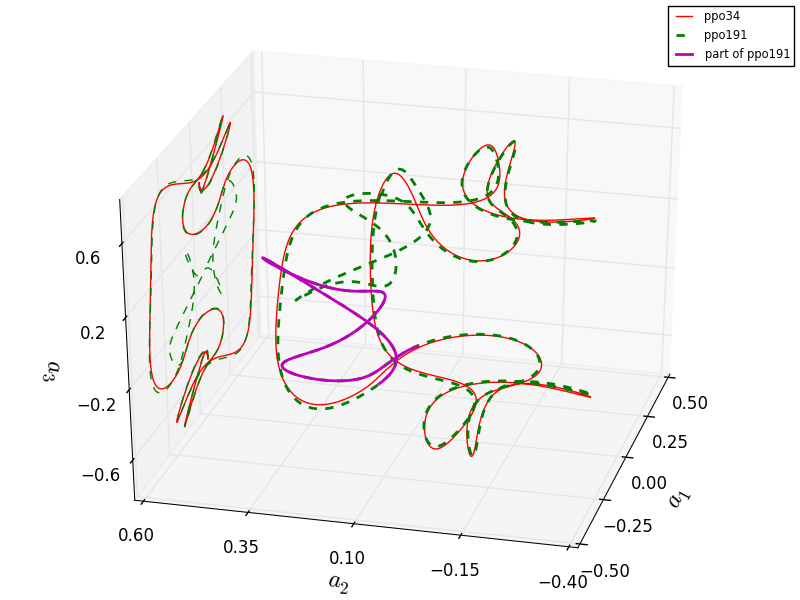
\includegraphics[width=1.0\textwidth]{ppo34ppo191.png}
	    \caption{
The orbit \cycle{ppo34} and \cycle{ppo191}. The purple part is a part of
\cycle{ppo191}, which I suspect has a \po\ close to it. The figure in
plane $a_{2}=0.8$ is  	a projection of the 3D figure.
	    }
	    \label{fig:ppo34ppo191}
    \end{figure}

    \begin{figure}[h]
    \centering
	    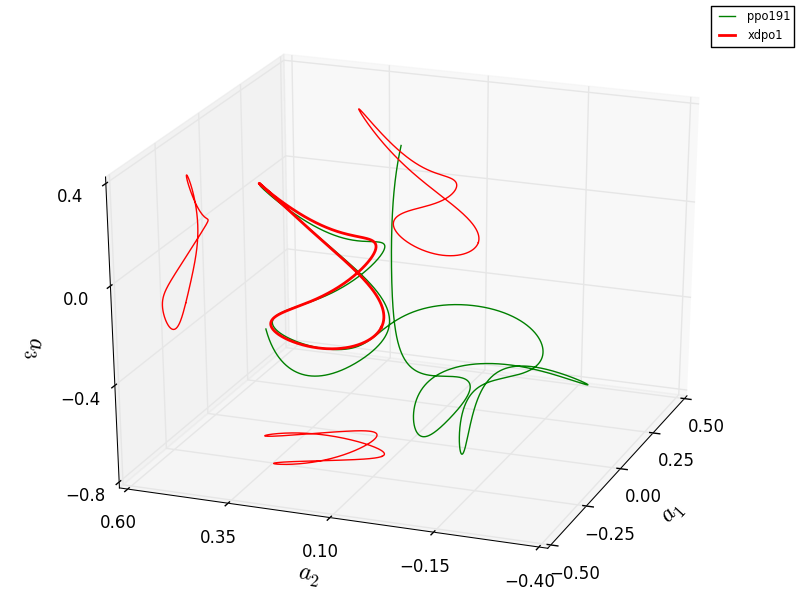
\includegraphics[width=1.0\textwidth]{xdpo1ppo191.png}
	    \caption{
The new \po\ \cycle{xdpo1} found by \LMa\ and its projection onto three
Fourier mode $[\ssp_i,\ssp_j]$ planes. The blue curve is a part of orbit
\cycle{ppo191}, which is used here to show the shadowing of these two
orbit.
	    }
	    \label{fig:xdpo1ppo191}
    \end{figure}


The initial condition for \cycle{xdpo1} is recorded in file \\
\texttt{siminos/xiong/matlab/data/xdks22ppo\_ve.mat},
which also contains the Floquet exponents and {\cLvs} for these orbits.
I have posted three videos to show the dynamics of these three orbits:
the 1st and 2nd Floquet vectors of
the pre-periodic orbit \cycle{ppo34}
\YTlink{www.youtube.com/watch?v=_7GYSWUhjU0}
\Xiong{2014-01-30}{Kazz: just to comment, I cannot play these Youtube videos... it just says "error".}
the pre-periodic orbit \cycle{ppo191}
\YTlink{www.youtube.com/watch?v=HSwF4FHcKP8},
and of
my first new \KS\ \po\
\cycle{xdpo1}
\YTlink{www.youtube.com/watch?v=KsKJlqanhzI}.
Click on the little gear, lower edge of the video, and increase
the resolution.

	\begin{table}[h]\small
	        \centering
                \rowcolors{1}{green}{pink}
                \begin{tabular}{ | c | c| c| c |}
		\hline
		   &  \large{\cycle{ppo34}}  	   &\large{\cycle{ppo191}} 	      & \large{\cycle{xdpo1}}       \\
		$\period{p}$ &  65.168     & 95.622		      &  28.661			 \\
		1  &  0.0906415303143404   & 0.163519387385378        &  0.310946570410124    \\
		2  &  7.6807244834054e-13  & -8.87742735450937e-10    &  1.82695233692736e-08 \\
		3  &  -3.96234572385144e-08& -2.92395682922365e-08    &  -1.00208509640834e-08      \\
		4  &  -0.0310548938604484  & -0.0880662661179373      &  -0.121543448733821         \\
		5  &  -0.179258937912979   & -0.153663430732254       &  -0.201501379498644         \\
		6  &  -0.256774704335013   & -0.288439007830585       &  -0.292650836258473   \\
		7  &  -0.27734427136977    & -0.297070591590133       &  -1.343131346286978   \\
                8  &  -0.32029818451026    & -0.324769085942675       &  -0.343131346286978  \\
              \end{tabular}
	      \caption{
Real parts of Floquet exponents for pre-\po s \cycle{ppo34},
\cycle{ppo191} and the \po\ \cycle{xdpo1}. For \cycle{ppo34} and
\cycle{ppo191}, period refers to the prime period. As \cycle{xdpo1} is
not self-dual under reflection, its prime period is the the whole period.	
	      }
	      \label{tab:floquet_exponents_ppo34ppo191xdpo1}
	\end{table}

\refTab{tab:floquet_exponents_ppo34ppo191xdpo1} gives the periods of
these three orbits and their Floquet exponents. The marginal exponents
are much more accurate than my in previous calculations because the
initial conditions for these orbits are refined by \LMa. As the two
shorter orbits shadow the longer one, the leading Floquet multiplier of
the long orbit is approximately a product of the Floquet multipliers of
the two shorter ones, so we expect:
	\begin{equation}
		\period{l}\,\eigRe[l]
         \approx \period{s1}\,\eigRe[s1]+\period{s2}\,\eigRe[s2]
    \,,
	\label{eq:relationorbits}
	\end{equation}
where $\eigRe[i]$ are the real parts of Floquet exponents. I checked this
relation for the first exponent, and I find the relative error is just
around 5\% ; therefore, we can predict the largest Floquet exponent of a
\po\ if we can find two or more shorter \po s to shadow it, which is
practically useful because calculating Floquet exponents is expensive
for long orbits.

However, relation \refeq{eq:relationorbits} is not satisfied by
other Floquet exponents
\Xiong{2014-01-30}{Kazz: I found it a sound and interesting observation.}.


\subsection{Very short time Lyapunov exponents}

Pre-\po s \cycle{ppo34} and \cycle{ppo191} are self-dual under reflection
symmetry, while orbit \cycle{xdpo1} maps into its twin.
\refTab{tab:floquet_exponents_ppo34ppo191xdpo1} shows that \cycle{xdpo1}
has two marginal exponents, one for perturbations along the orbit, and
the other for the \SOn{2} perturbations in the group tangent direction;
the continuous symmetry sweeps out a torus of \po s (not \rpo s).

\begin{description}

\item[2014-01-10 Xiong Ding]
{Video} \YTlink{www.youtube.com/watch?v=KsKJlqanhzI}
shows
that the local Floquet exponents for the 1st and 2nd {\cLvs}
repeat twice in one period. Therefore it should have some ``reflection''
symmetry. Am I right?

\item[2014-01-12 Predrag] Not if this is a pair of \po s related by
the reflection.
But I remember from \refref{Christiansen97} that the remanent of the $\SOn{2}$
circular group orbit restricted to the anti-symmetric subspace are two
points related by $\Zn{2}$. This might be the source of this reflection
symmetry. Presumably once you learn how
to slice and also quotient the discrete symmetry $\mathbf{Z}_2$, these will
be half period and much less wiggly.

\item[2014-01-12 Predrag]  What `local Floquet exponent' might be?
Eigen-exponent of a finite time Jacobian multiplier? That has no
meaning...

\item[2014-01-13 Xiong to Predrag] I am sorry the misleading term I created.
 I got the eigenvectors of Jacobian
matrix ({\cLvs}) and evolved them along the orbit. The logarithm of
expansion rates of {\cLvs} are recorded:

\begin{equation}
  \label{eq:locallyapunov}
  \lambda^{(i)}(t)=\frac{1}{h}\ln \frac{|v^{(i)}(t+h)|}{|v^{(i)}(t)|}
\,,
\end{equation}
where $h$ is the time step and index $i$ refers to the $i_{th}$ {\cLv}.
So, it should be the `local Lyapunov exponent'. Right?

\item[2014-01-13 Predrag] It looks like you are computing an arbitrary,
\emph{very} short time finite time Lyapunov exponent. Why would one do
that? This has no invariant meaning. It makes no sense at all to me. You
might just as well plot the eigenvalues of $\Mvar + \transp{\Mvar}$ as
function of $\ssp(\zeit)$, which is s symmetrized generalization of the
1\dmn\ derivative $\partial_x \vel(x)$ to higher dimensions. Would be
more useful to plot something like the angles $\cos(\theta_{ij}(\zeit))$
between Floquet eigenvectors $\{\jEigvec[i], \jEigvec[j]\}$.

Write up the definition of the finite time Lyapunov exponents, if you
have not done it yet someplace earlier in your blog notes. You can clip
\&\ paste the definition from
\\
\texttt{dasbuch/book/chapter/Lyapunov.tex}:
If the
unit vector $\unitVec$, $\norm{\unitVec} =1$ at the initial time
is aligned along the $i$th {principal stretch},
\(
\unitVec = {u}^{(i)}
\,,
\)
then the corresponding finite-time
Lyapunov exponent (rate of stretching) is given by
\beq
\Lyap_j(\xInit;\zeit) =
%\max_{\|\unitVec\|=1}
    \Lyap(\xInit,{u}^{(j)};\zeit)
    = \frac{1}{\zeit}\ln\sigma_j(\xInit;\zeit)
\,.
\ee{e:ftLyapStretch}
You would do me a great favor if you reread critically the Lyapunov
chapter in \textbf{ChaosBook.org}, edit/suggest improvements that would
make it easier to read :)

\item[2014-01-30 Kazz] Though I cannot say right now how such finite-time Lyapunov exponents can be used, I wouldn't say this is meaningless... This obviously gives local stretching rate of each Floquet vector. Therefore, I actually think that Xiong's speculation is correct... non? By the way, Xiong, you can directly check it simply by looking at the vector at time 0 and at a half of the period.


\end{description}

\subsection{Hyperbolicity of Floquet vectors}

According to Kazumasa~\etal\ previous work, hyperbolicity properties of
{\cLvs} have been used to
distinguish between the subspace of `{\entangled} Lyapunov modes' and
the subspace of contracting `{\transient} Lyapunov modes'. Their crucial observation
is that the {\transient} Lyapunov modes are nearly perpendicular to {\entangled} modes
and nearly perpendicular among themselves; however, the {\entangled} modes can be
tangential among themselves at some points. This observation indicates that
perturbations in the contracting {\transient} subspace  die out
 without any effect on
other modes.
But, since we can calculate the eigenvectors of Jacobian matrix, do Floquet
vectors have the similar properties as Lyapunov modes%
    \PC{I feel intense headache coming on - we talked about it on Friday
    and I thought we agreed. `Lyapunov modes' as used by Kazumasa and
    Hugues (I cite their definition in ChaosBook) is the set of both
    {\cLvs} and associated Lyapunov exponents of a given infinite time
    orbit, taken together. You have shown me that you have checked that
    for a \po\ the infinite time Lyapunov exponents do converge to
    $\eigRe[j]$, the real parts of Floquet exponents (evaluated on a
    single period), and you said were going to write that up (including
    the explanation that for complex pairs only the sum converges to
    $\eigRe[j]$, while each one singly oscillates with $\eigIm[j]$).  The
    only difference is that `Lyapunov' calculation converges only in an awkward and
    unnatural limit, convenient only for Oseledec rigorous mathematics, while
    Floquet is the natural object in dynamics.

    So what ``similar properties?'' For a \po\ `Lyapunov mode'
    \underline{is} identically the Floquet vector + the real part of the
    Floquet exponent, $[\jEigvec[j],\eigRe[j]]$.
    }
when applied to periodic orbits?

\begin{figure}[h]
  \centering
  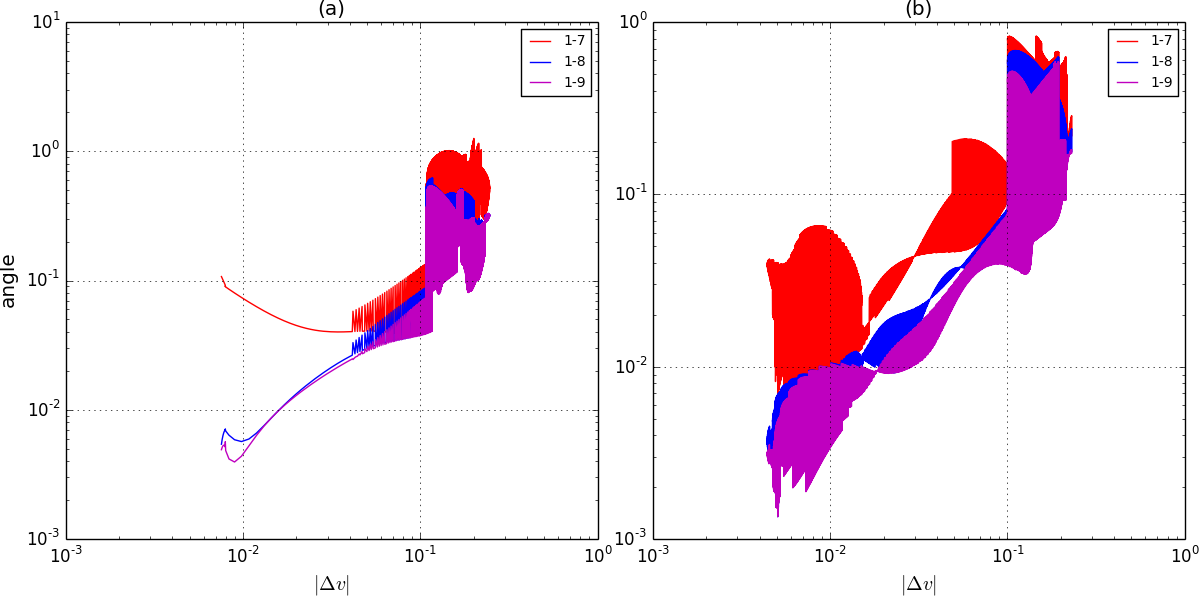
\includegraphics[width=1.0\textwidth]{ang789.png}
  \caption{The angle between the difference vector
  \refeq{eq:differencevector} and the subspace spanned by the first few
  Floquet vectors as a function of the Euclidean length $\norm{\Delta
  u(\zeit)}$ of the difference vector. (a) In the intervals where the
  pre-periodic orbit \cycle{ppo191} approaches \cycle{ppo34}, the first 7
  Floquet vectors are insufficient, but the first 8 Floquet vectors
  span the space that contains Delta $u(\zeit)$ to a good accuracy. (b)
  Pre-periodic orbit \cycle{ppo191} approaches \cycle{xdpo1}.
  }
  \label{fig:ang789}
\end{figure}

I take the re-periodic orbit \cycle{ppo191} together with \cycle{ppo34} and \cycle{xdpo1}
which shadow it. The difference vector is defined
as
\begin{equation}
  \label{eq:differencevector}
  \Delta u(\zeit)=u_{p_1}(t)-u_{p_2}(t-\tau)
\end{equation}
where, $u_{p_1}(t)$ and $u_{p_2}(t-\tau)$ are \statesp\ locations  of
 \cycle{ppo191} and \cycle{ppo34}( or \cycle{xdpo1}) respectively, and
parameter $\tau$ is chosen to minimize the Euclidean norm $\norm{\Delta u(t)}$.

If subspace spanned by `{\transient} Floquet modes' is disentangled from the
subspace spanned by `{\entangled} Floquet modes', then any perturbation along
the {\transient} Floquet modes will die out soon because its large negative
Floquet exponents; therefore, the difference vector should be within the
subspace of `{\entangled} Floquet modes'.

\begin{figure}%[h]
  \centering
  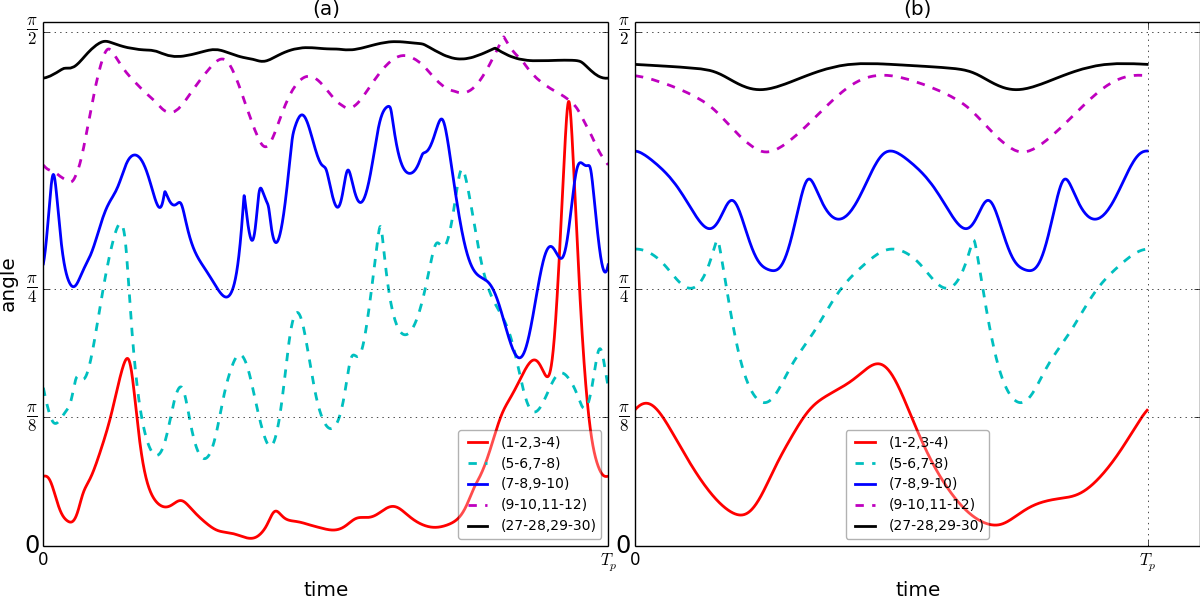
\includegraphics[width=1.0\textwidth]{angle_subspace.png}
  \caption{
  Smallest principal angles between subspaces spanned by Floquet vectors.
  (a) Pre-periodic orbit \cycle{ppo34}. (b) \po\ \cycle{xdpo1}
  }
  \label{fig:angle_subspace}
\end{figure}

\refFig{fig:ang789} shows the angle between the difference vector and
the hyperplane spanned by the first $N$ Floquet vectors for two pairs
of orbits.
    \PC{angle in what units? Degrees? Radians? If you plot $\sin$ of the
    angle instead, you do not have to say. Do you define this angle
    anywhere? Floquet vectors of which \po? Is the result similar for either?}
When $N=7$, the angle grows when the difference vector becomes shorter,
which indicates that the first 7 Floquet vectors cannot span the
{\entangled} subspace. However, when $N=8$ or $N=9$, the angle decreases
exponentially
\Xiong{2014-01-30}{Kazz: not exponential, but linear (slope = 1), as expected for the angle here.} as the two pre-periodic orbits get closer, and the
difference between the $N=8$ and case with $N=9$ cases is small. So,
could we say the first 8 Floquet vectors span the {\entangled} subspace?
At least for these three particular orbits?
    \PC{I do not get the oscillations in the solid color regions, and I
    do not get  \reffig{fig:ang789} at all - what do these blobs mean?
    Isn't there a unique $\tau$ for each value of $t$, \ie, each point
    $u_{p_1}(t)$ on the \po\ $p_1$?}
    \Xiong{2014-01-30}{Kazz: excellent! I agree about your conclusion here (and this number 8 is what we would expect from the physical dimension for ergodic trajectories!), though it's true that the blobs Predrag pointed out are worrying and we have to figure out what they are (and whether the result here is reliable). The definition of the \entangled subspace is not clear. Shall we \textit{define} the entangled subspace for a given pair of periodic orbits by the way you did here? I'd also like to see the fraction of time at which the two orbits are separated at each distance $|\delta v|$ in this figure. The averaged angle for small $|\delta v|$ must be obtained only from a few number of data (time steps), right?}

As we are interested in the intervals of small separations between nearby
orbits, perhaps the {\entangled} dimension can be detected by
investigating the neighborhood of a single periodic orbit. That is what
one does in the long time simulations of a single ergodic orbits; one
studies angles between its {\cLvs}, not its distances to other orbits or
it recurrences. \refFig{fig:angle_subspace} shows the angles between
different subspaces spanned by Floquet vectors for two of the shortest
periodic orbits of $L=22$ \KS.
        \PC{OK, angle is in radians. Do give a clear definition of the
        `principal angles'. Maybe plot $\sin$ on the logarithmic plot?}
While two \po s are insufficient to make a statistical analysis of small
angles, presumably what we care about are the minima along a given orbit,
as these are the instants where perturbation along one of the {\cLvs} is
most entangled. In these examples the leading {\cLvs} are most entangled,
while {\cLvs} beyond the 8th one are always quite orthogonal to the rest,
in agreement with the long-time simulations.

\begin{description}

\item[2014-01-30 Kazz] Excellent!! This is really what we wanted to see! However, it's too early to conclude that the physical dimension of ergodic trajectories can be estimated from a pair of periodic orbits: it may be just a coincidence! What we really have to do is to elucidate in what conditions the entangled subspace dimension of a given pair of periodic orbits gets equal to the phydical dimension. We (Hugues and I) speculate that hyperbolicity of periodic orbits matters. How hyperbolic are the two orbits you used here? In other words, what is the minimum angle between two entangled {\cLvs} (i.e. two of the first eight {\cLvs}) ? If these orbits are rather hyperbolic, try to find a pair of nearly non-hyperbolic orbits (or a pair of a hyperbolic orbit and a nearly non-hyperbolic one) and measure the same thing. What do you get?



\item[Xiong Ding 2014-04-15]

  \begin{figure}[h]
    \centering
    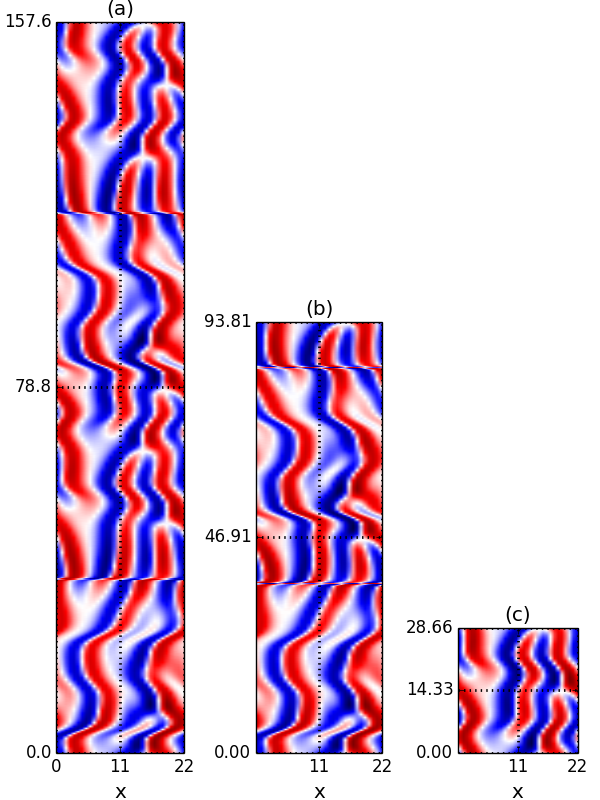
\includegraphics[width=0.8\textwidth]{state69_13_2_SO2fm1}
    \caption{State space onfiguration of (a) \cycle{ppo69}, (b)
      \cycle{ppo13} and (c)
      \cycle{ppo2} after quotienting out \SOn{2}\ symmetry by the first
      Fourier mode slicing. All of them are evolved for $2T_{p}$ with $T_{p}$
      the prime period respectively.
    }
    \label{fig:state69_13_2_SO2fm1}
  \end{figure}

I repeated the same procedure as above on another pair of shadowing orbits: \cycle{ppo13} and \cycle{ppo69}. Two cases are considered here depended
on the different definitions of difference vector, one of which does not
consider \SOn{2}\ symmetry while the other does.

\paragraph{The first case}
In this case, difference vector is defined as
$\Delta u(t_1)= u_{p_1}(t_1)-u_{p_2}(t_2)$ with $t_2$ minimizes the
Euclidean norm of $\Delta u(t_1)$.

\begin{figure}[h]
  \centering
  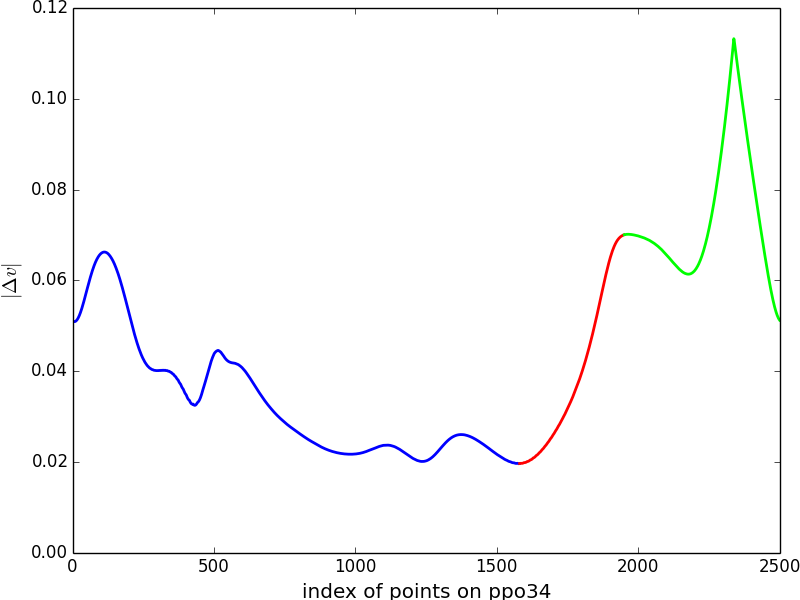
\includegraphics[width=1.0\textwidth]{dis_69_13}
  \caption{Euclidean norm of the difference vector along \cycle{ppo13}.
    Red and blue lines represent the part when the two
    orbits(\cycle{ppo13} and \cycle{ppo69}) shadow each other,
    and green curve represents the part at which these two orbits diverge
    from each other. The red part is chosen as the incidence window.
    In this plot \SOn{2}\ symmetry has not been considered.
  }
  \label{fig:dis_69_13}
\end{figure}

\begin{figure}[h]
  \centering
  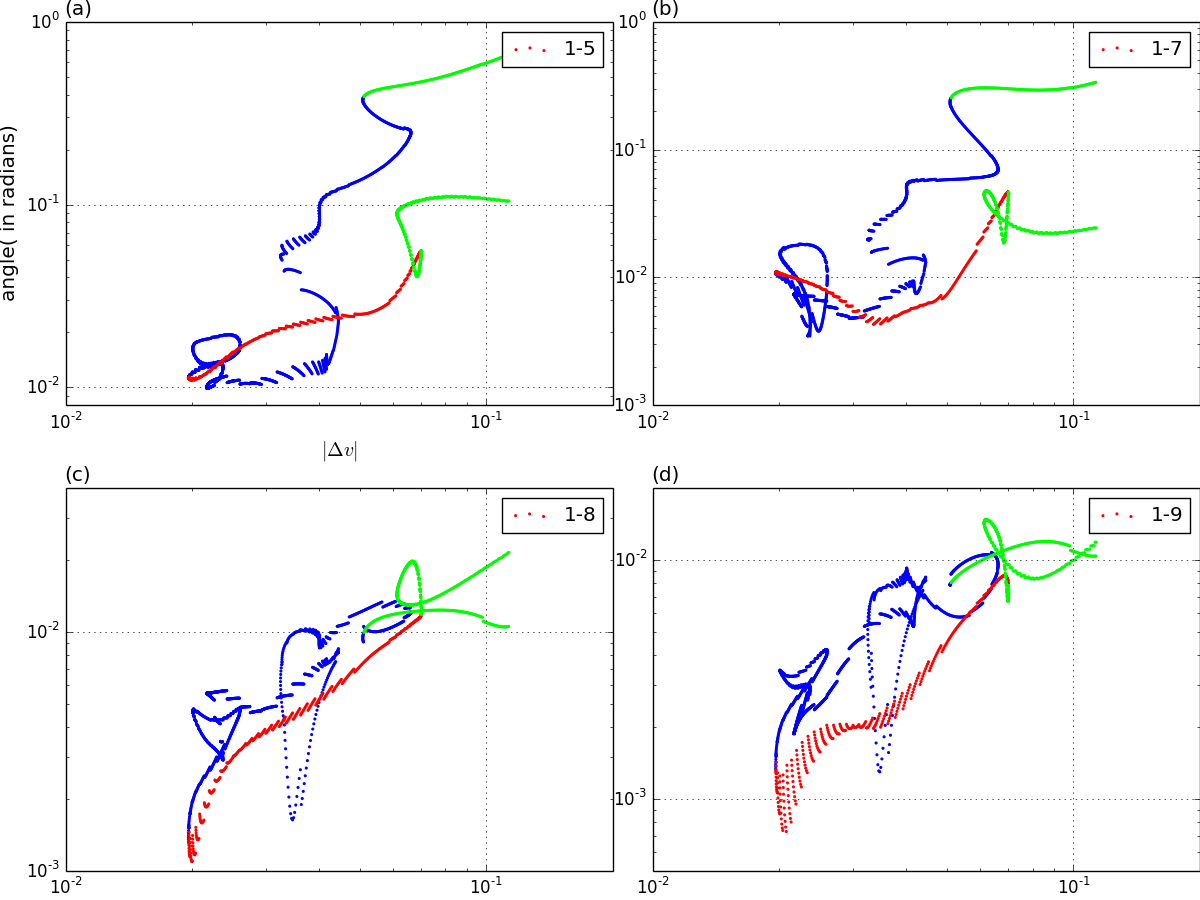
\includegraphics[width=1.0\textwidth]{dis_ang_69_13}
  \caption{
    Angle between difference vector and the subspace spanned by
    the first few Floquet vectors. Orbit $p_2$ approaches orbit
    $p_1$. First few Floquet vectors
    of orbit $p_1$ are used to span the subspace. In this
    case, $p_2$ is \cycle{ppo69} and $p_1$ is \cycle{ppo13}.
    (a) (b) (c) and (d) use 5,7,8 and 9 first Floquet vectors
    respectively to span the subspace. Red, green and blue dots
    correspond to the same part of incidence in \reffig{fig:dis_69_13}. In this plot \SOn{2}\ symmetry has not been
    considered.
    The discontinuity in the plot does not come from
    code error. When trying to
    find difference vectors, the distance is minimized, so the
    direction of difference vector may changed a little abruptly
    at some moment, especially when the distance is really small.
  }
  \label{fig:dis_ang_69_13}
\end{figure}

\paragraph{The second case} \SOn{2}\ symmetry is taken into account.
The definition of difference vector is
\beq
\Delta u(t_1)= u_{p_1}(t_1)-g(\theta)u_{p_2}(t_2)
\,,
\ee{eq:difvec_SO2}
where $\theta$ and $t_2$ are chosen to minimize the Euclidean
length of $\Delta u(t_1)$. Here $g(\theta)$ is an \SOn{2}\ group transformation
and $p_1,p_2$ are two periodic orbits. In our case, $p_1$ is \cycle{ppo13}
and $p_2$ is \cycle{ppo69}.

I have read \refsect{sect:DraftBlog}, about the debate
between Evangelos and Kazz on the issue of determining
optimal shift when defining the difference vector.
It seems that Kazz tried to align the second Fourier
modes of a ergodic trajectory and a periodic orbit, so
he thought his route is approximate. As pointed out by him
(2011-08-11 Kazz 2 Evangelos), the reason he did not use the definition
\eqref{eq:difvec_SO2} is a pure computational issue: this definition
is very expensive numerically. I sincerely sympathize with him because
I encountered the same problem at the beginning.  Everyone including me
believes that if the optimal shift is determined between two points, then
Newton method will easily generate all the optimal shifts between other
points because the flow is continuous and the only variable is the group
angle $\theta$ , but actually the situation is
more complicated than we thought because we cannot predict which local
minimal point the Newton method will converge to. For example,
at point $x(t)$, take $\theta_1(t)$ and $\theta_2(t)$ as the two local
optimal shifts and $\theta_1(t)$
is also the global minimal. The Newton method converges
to $\theta_1(t)$, which is good. We now use $\theta_1(t)$ as the initial
condition to computer the optimal shift at next step $x(t+dt)$, and
Newton method probably converges to $\theta_{1}(t+dt)$; however, we could
not claim that $\theta_{1}(t+dt)$ is the global optimal shift because
$\theta_{2}(t+dt)$ may generate smaller Euclidean distance between the
two new points. What's more, I cannot find a way to predict when this
situation will happen. Initially, I wrote a Matlab script to implement
\eqref{eq:difvec_SO2}, but gave up soon because I lost my patience.
Finally, I turned to C with optimization and parallelization. Now it
is tolerable at least for short orbits (trajectories).

I hope I understand the \refsect{sect:DraftBlog} discussion correctly.

\begin{figure}[h]
  \centering
  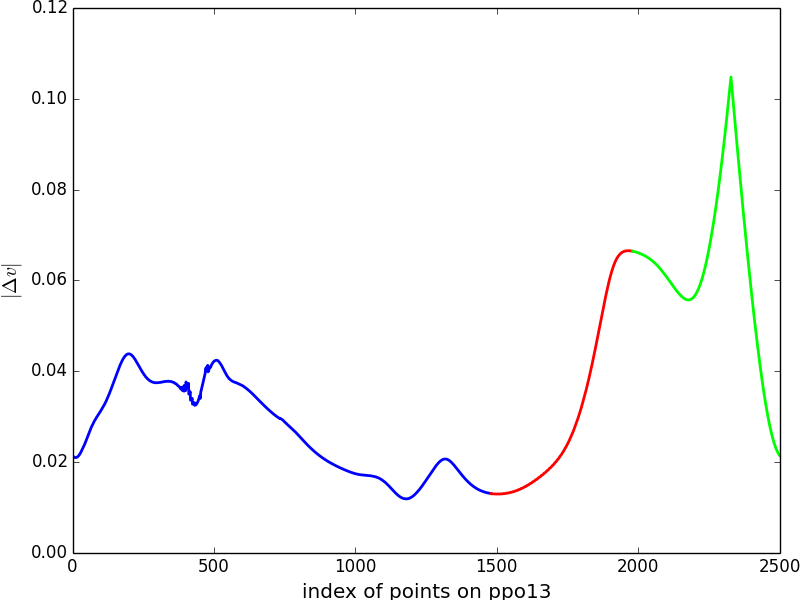
\includegraphics[width=1.0\textwidth]{dis_69_13_SO2}
  \caption{Norm of the difference vector along \cycle{ppo13}.
    Red and blue lines represent the part when the two
    orbits(\cycle{ppo13} and \cycle{69}) shadow each other,
    and green curve represents the part at which these two orbits diverge
    from each other. The red part is chosen as the incidence window.
    In this plot \SOn{2}\ symmetry has been considered.
  }
  \label{fig:dis_69_13_SO2}
\end{figure}

\begin{figure}[h]
  \centering
  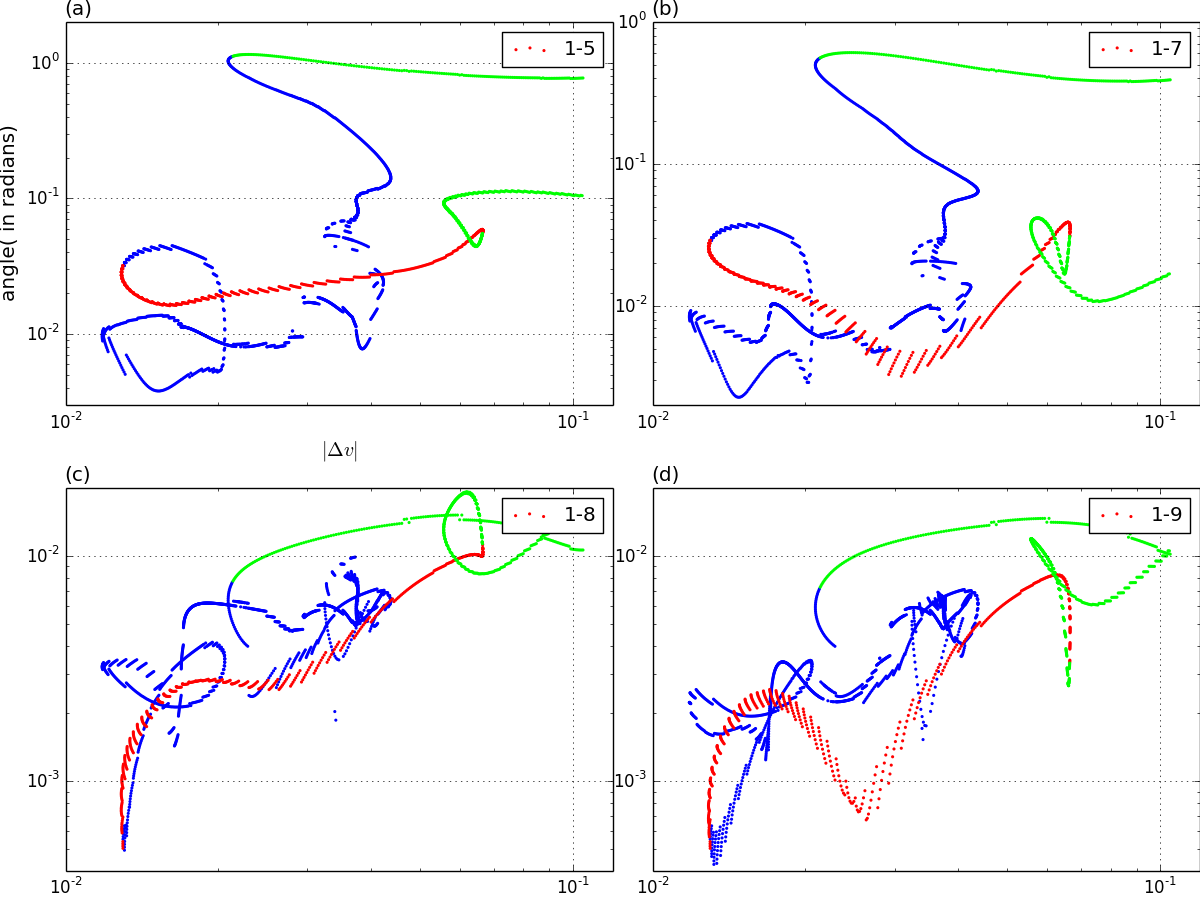
\includegraphics[width=1.0\textwidth]{dis_ang_69_13_SO2}
  \caption{
    Angle between difference vector and the subspace spanned by
    the first few Floquet vectors. Orbit $p_2$ approaches orbit
    $p_1$. First few Floquet vectors
    of orbit $p_1$ are used to span the subspace. In this
    case, $p_2$ is \cycle{ppo69} and $p_1$ is \cycle{ppo13}.
    (a) (b) (c) and (d) use 5,7,8 and 9 first Floquet vectors
    respectively to span the subspace. Red, green and blue dots
    correspond to the same part of incidence in
    \reffig{fig:dis_69_13_SO2}. In this plot \SOn{2}\ symmetry has been
    considered.
  }
  \label{fig:dis_ang_69_13_SO2}
\end{figure}

\clearpage
\subsection{Statistical results}

For two subspaces $\mathcal{F}\in\pS$, $\mathcal{G}\in\pS$ of a space
$\pS$ equipped with an inner product, the principal angles (canonical
angles) $\theta_k$ between vectors $u\in \mathcal{F}\,, v\in \mathcal{G}$,
\[
\cos(\theta_k) = \max
u^\top v = u_k^\top v_k
\,,
\]
subject to restriction
\[
||u|| = ||v||=1\,, u^\top u_i = 0\,, v^\top v_i = 0\,, i = 1,\cdots,k-1
\,,
\]
provide information about the relative position of $\mathcal{F}$ and
$\mathcal{G}$ inside the full space\rf{Knyazev02}.
The number of principal angles is
$q = \min(\dim\mathcal{F}, \dim\mathcal{G})$,
and the smallest one is the smallest angle that can be spanned by two
arbitrary vectors, one from each subspace. For example, for two perpendicular
planes inside a 3d space, the two principal angles are $0$ and
$\pi/2$.  On the other hand, if one subspace is one-dimensional, then
the unique principal angle refers to the projection angle of a vector
to a subspace. Knyazev and Argentati\rf{Knyazev02} give a simple algorithm
to calculate
principal angles,
\[
\theta_k = \arccos(\sigma_k)\;, k = 1,2,\cdots, q
\,,
\]
with
\[
svd(Q_F^\top Q_G) = diag(\sigma_1, \cdots, \sigma_q)
\,,
\]
where $svd$ refers to singular value decomposition. $Q_{F}$ and $Q_G$ are
orthonormal basis inside each subspace. Numerically, the algorithm can
be implemented as a singular value decomposition after two QR
decompositions.

In order to distinguish the disentangled and entangled subspace in \KSe,
the general idea is to determine the likelihood of random
small perturbation in one subspace evolving into the other
subspace as time goes on. \refRef{YaTaGiChRa08} uses CLVs to investigate
the embedding dimension of the global attractor of KS system; here,
on the other hand, we turn to Floquet vectors associated
with periodic orbits since they govern the dynamics inside the
tangent space, so for our purpose, the obvious way is to study the smallest
principal angle between subspaces spanned by different combinations
of Floquet vectors along these orbits.

\cycle{ppo} and \cycle{rpo}, with periods $\period{p} < 100$, are used as samples in
 \reffig{fig:statistic_angle_rpoppo}. We put threshold index at $7, 8, 9$
and record the smallest principal angles along each orbit. When the 7th and
8th Floquet vectors form a complex conjugate pair, then the indices are
changed to $6, 8, 9$. The same goes for other indices.

We first observe
that 8th and 9th never form a conjugate pair, but other possibilities
occurs for some orbits. Also from (a) and (c) in
 \reffig{fig:statistic_angle_rpoppo}, we can see that
the angle mostly stays near zero when the 8th is separated
from the first seven Floquet vectors, but immediately exclude 8th from the
remaining subspace, the distribution shift to large angles, which means
that the first 8 dimensions are closely related to each other but are
quantitatively separated from the remaining dimensions. Also there is
a peak accumulation at larger angle for index equal to 8 and 9.
The angles between vectors are plotted in (b) and (d). The
angles for vectors inside the entangled zone have fairly flat distribution
from 0 to $\pi/2$, but angle between vectors from entangled and
disentangled space or both from disentangled space mainly accumulate
near $\pi/2$.

\begin{figure}[h]
  \centering
  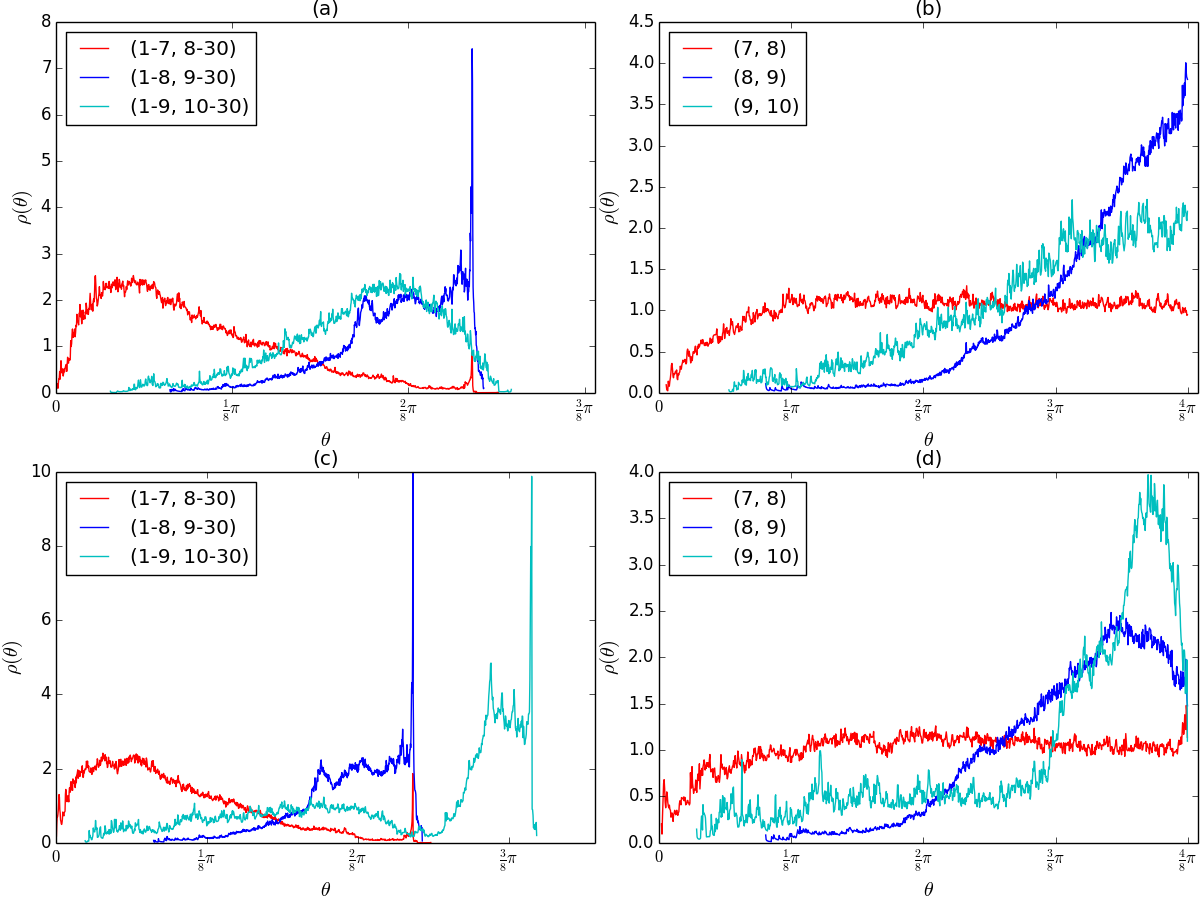
\includegraphics[width=1.0\textwidth]{statistic_angle_rpoppo}
  \caption{
    (a)(b) Smallest principal angle distribution for the first
    240 pre-periodic
    orbits ($T_p < 100$). Number in the parentheses donate the indices
    of Floquet vectors that span the corresponding subspace. $y$-axis
    is the normalized distribution, and $x$-axis is the span of angles.
    (c)(d) The same graph for the first 239 \rpo s with
    $T_p < 100$.
  }
  \label{fig:statistic_angle_rpoppo}
\end{figure}


Another way to investigate the local dimension of \KS\ system is to
find how good enough the first few Floquet vectors can expand the
difference vector which is defined as
\[
\Delta x = \hat{x}(t_p) -\hat{x}_0
\,,
\]
where the hat means the vector is defined in \SOn{2}\ reduced space
(for simplicity, we choose the first Fourier mode slice), and $t_p$
denotes the time to evolve the state onto the {\PoincSec} defined by
template point $\hat{x}_0$ and the velocity field at $\hat{x}_0$.

The definition used here eliminates the importance of the two marginal
vectors in the full spectrum of Floquet vectors associated with each
orbit. In order to find how many dimensions are needed to fairly expand
the difference vector, Floquet vectors are first projected onto the 1st
mode slice and then projected onto the {\PoincSec}. A detailed
description abofout this technique is given in \refsect{sect:symm}.
Ergodic trajectories are obtained in the full state space and then
reduced in the 1st mode slice, after which, {\PoincSec} points are
collected.

\begin{figure}[h]
  \centering
  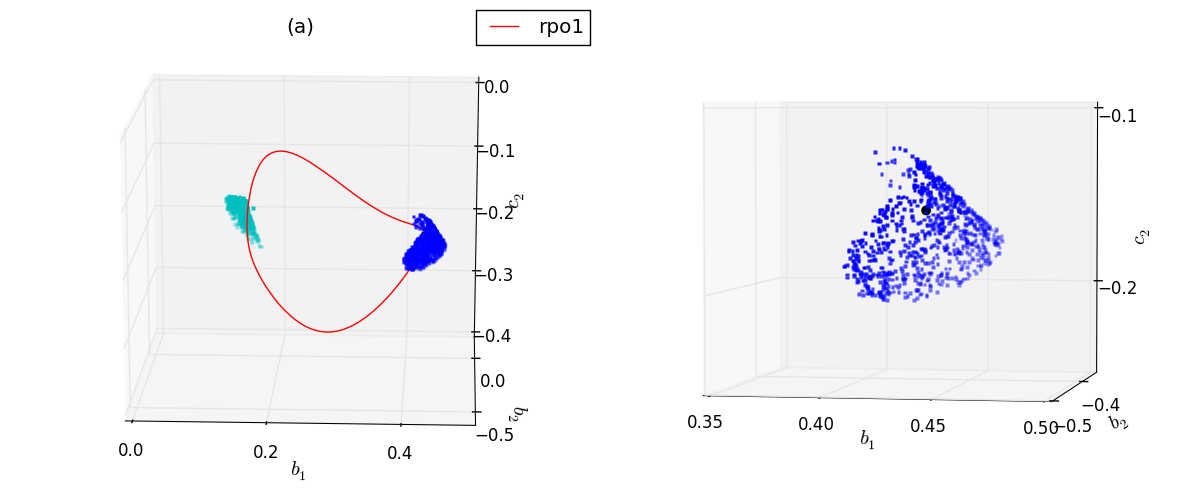
\includegraphics[width=1.0\textwidth]{poincare_intersection_rpo1}
  \caption{(a) \cycle{rpo1}(red) with the two sets of {\PoincSec s}
    (blue and cyan)
    points near the border and far away from the slice border. The points
    are generated from an arbitrary initial point on the attractor, and
    velocity field at the template point is used to define the {\PoincSec}. Only intersection points close enough to the template points
    are recorded. (b) the magnified version of the template point far away
    from the slice border (black point) and the intersection point around
    it (blue).
  }
  \label{fig:poincare_intersection_rpo1}
\end{figure}

\begin{figure}[h]
  \centering
  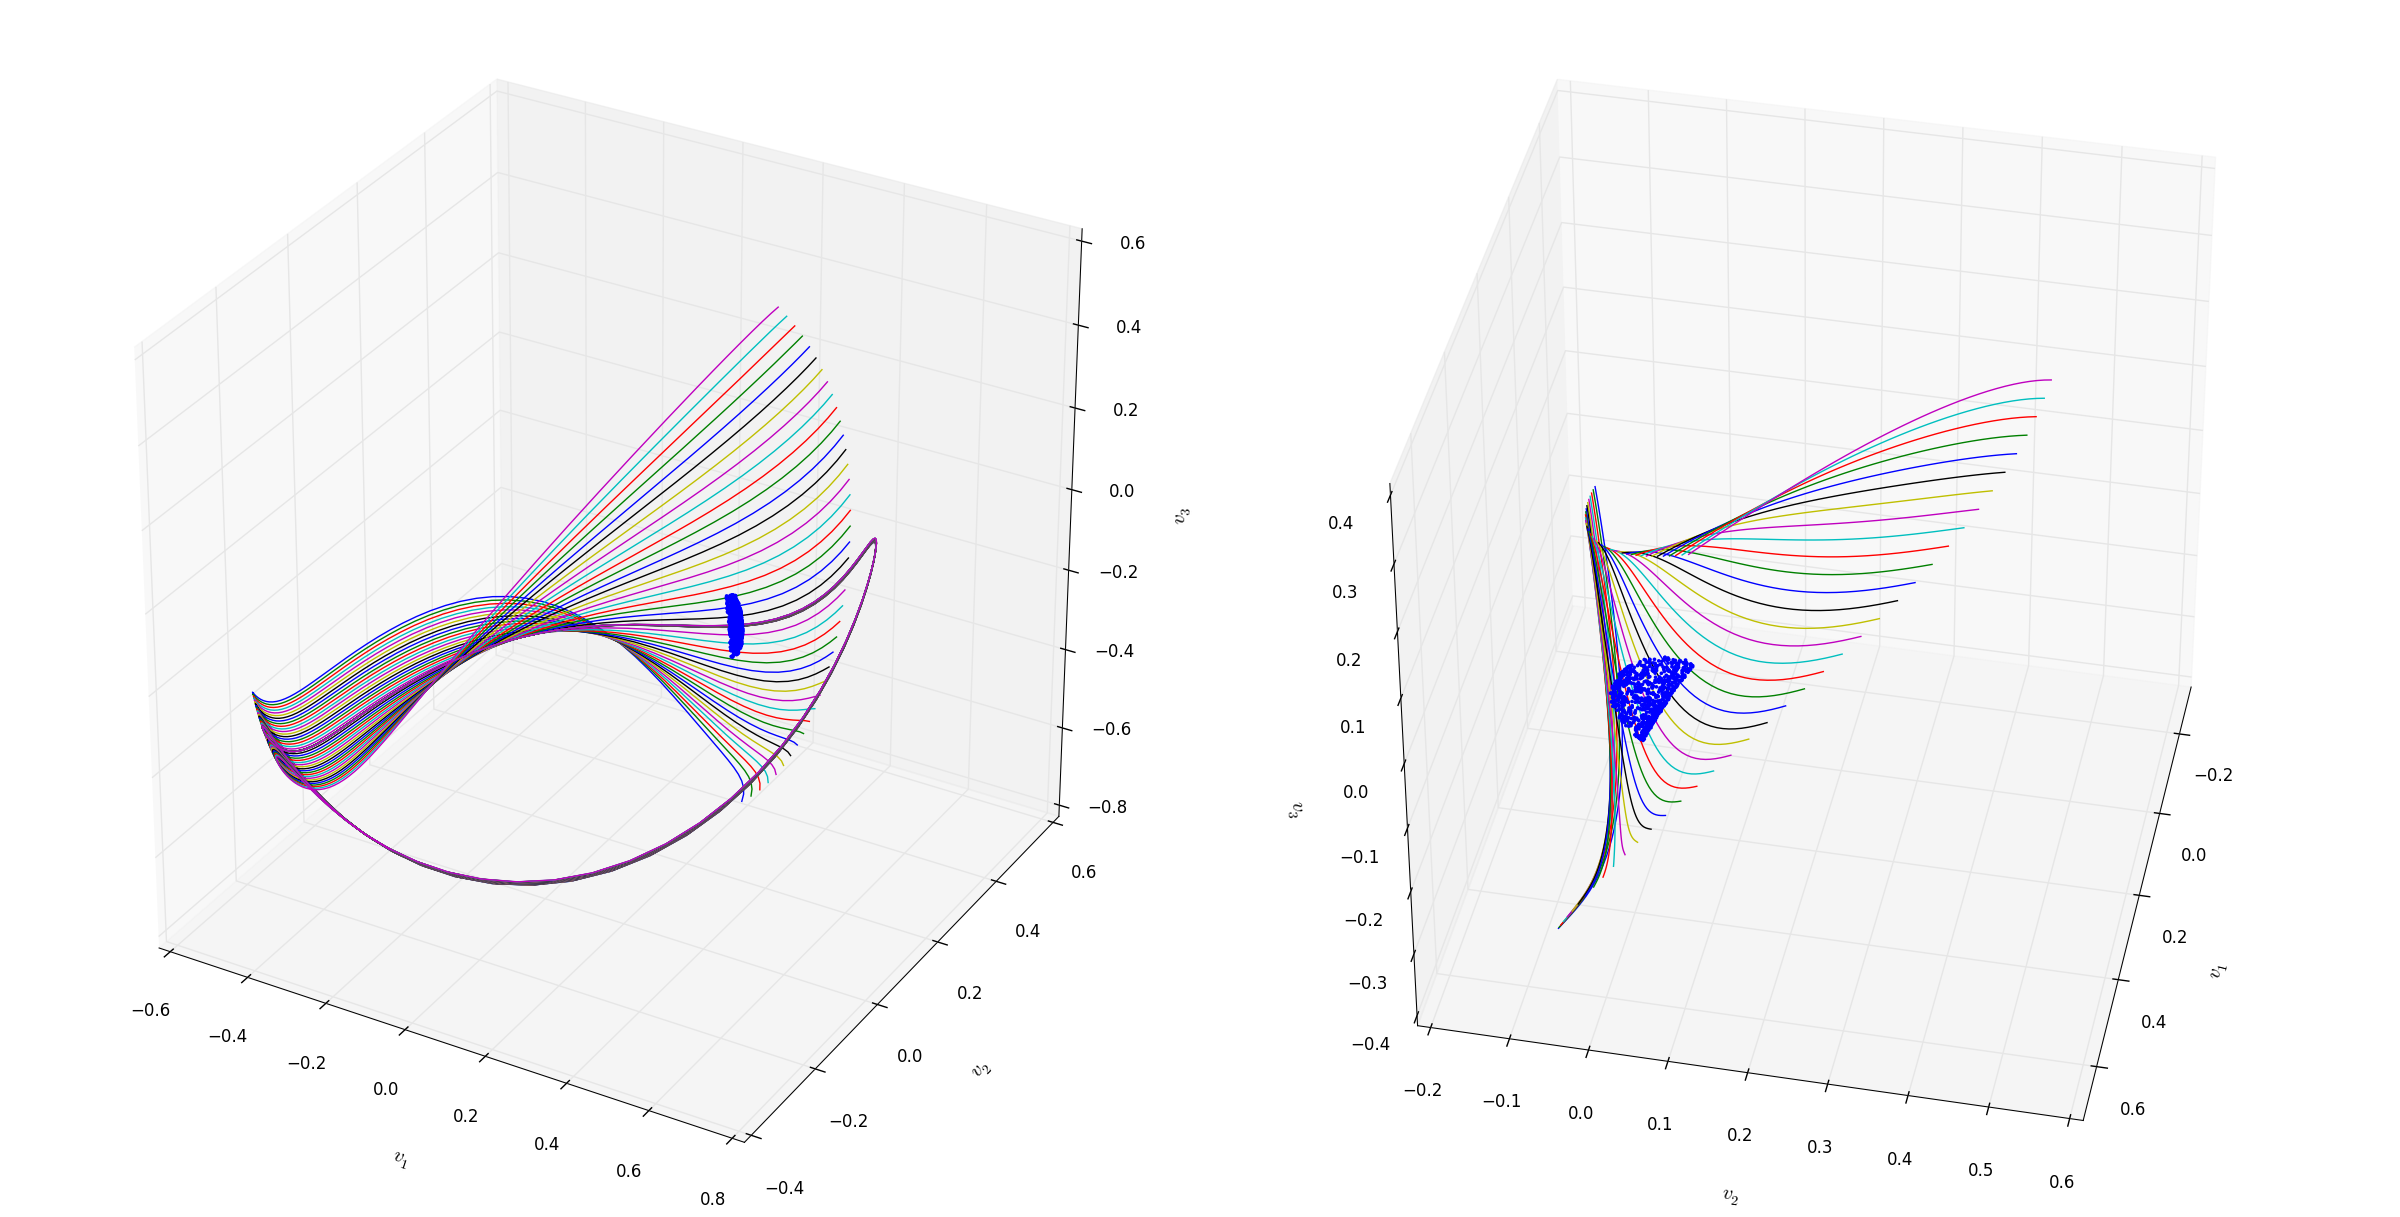
\includegraphics[width=1.0\textwidth]{manifold_rpo1}
  \caption{Unstable manifold of \cycle{rpo1} on the 1st mode slice. The
  axes $v_1$, $v_2$, $v_3$ are Floquet vectors $e_1$, $Im(e_5)$ and
  $Re(e_5)$. (b) is the same as (a) with a different angle of view.
}
  \label{fig:manifold_rpo1}
\end{figure}

We choose the farthest and closest point on an orbit as template point
to construct {\PoincSec} to demonstrated that \SOn{2} reduction will
not change the local structure in the full state space. On the other
hand, the velocity field at the two location are most likely parallel
to the slice border and thus the resulting {\PoincSec} is perpendicular
to the slice border. Our experience tells us that ergodic trajectories
tend to move around the slice border from time to time, so in this way,
we are more likely to get a lot of intersection points.

 \refFig{fig:poincare_intersection_rpo1} shows that when only 5 Floquet
vectors are used to span the subspace, the principal angle will not
diminish as we get closer to the template point, which means 5
dimensions are not enough to construct the local structure around the
template point. However, when one more Floquet vector is added, the
scenario changes immediately. As the distance decreases, the
corresponding principal angle decrease accordingly. Also, if more
dimensions are added, the scenario does not change qualitatively.
Therefore, we reach the conclusion that local dimension at these
template points is $6$ on the {\PoincSec} and 8 in the full state
space. Note that there is a distinct structure on the data collected.
It seems that the relation is linear, and the slope may indicate the
properties of the local structure, which are unknown to me. On the
other hand, the length of difference vectors ranges from 0.01 to 0.1
because of the extremely low probability to obtain intersection points
much closer to the template point along an ergodic trajectory. Maybe we
can get more convincing result if longer evolution time is employed.

\begin{figure}[h]
  \centering
  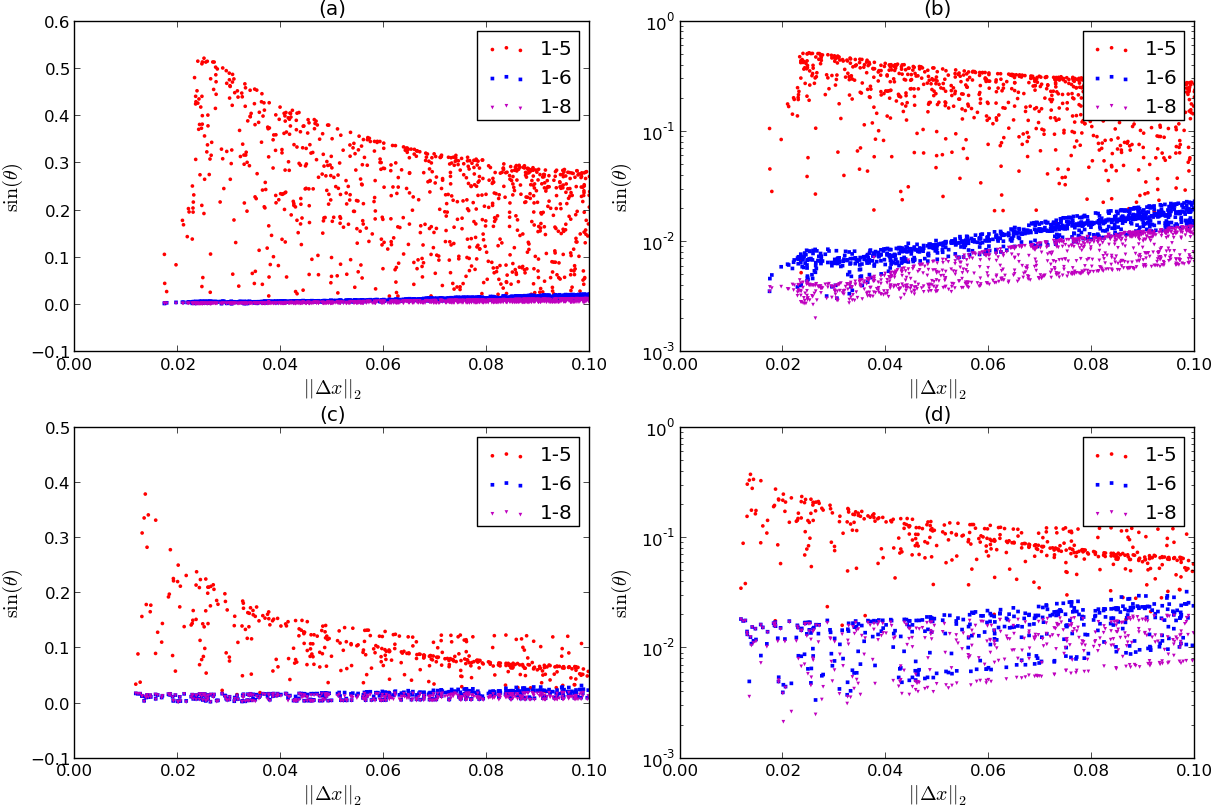
\includegraphics[width=1.0\textwidth]{ergodic_angle_rpo1}
  \caption{
    Principal angle between difference vector and subspace spanned by the
    first few Floquet vectors versus the Euclidean length of the difference
    vector. Difference vector is defined on the {\PoincSec} constructed
    from farthest/closet point on \cycle{rpo1} to slice border.
    The right side
    is the same figure as the left side with y-axis changed to log scale.
    The legend specifies how many Floquet vectors are used to construct
    the local subspace. Note the 7th and 8th Floquet vectors form a
    complex conjugate pair.
    (a) (b) Farthest point is chosen as the template point of {\PoincSec}. 885 points are collected.
    (c) (d) Nearest point is chosen as the template point of {\PoincSec}.  397 points are collected.
  }
  \label{fig:ergodic_dis_angle_rpo1}
\end{figure}

This experiment is conducted for other orbits.
\refFig{fig:ergodic_dis_angle2} shows similar results for several
other cycles. It clearly shows that the local dimension
is 8 for most state points. However, when I tried to do
the same experiment for \cycle{ppo4}, the result is different
from all the others as shown in figure. Although there is distinction
between the first 7 and 8 dimensions when expanding the difference
vector, the tendency of the movement of these intersecting
points is not along a
declining line when distance is getting smaller. I guess this
observation should indicate
a different local structure as was shown in
 \reffig{fig:ergodic_dis_angle2}.

\begin{figure}[h]
  \centering
  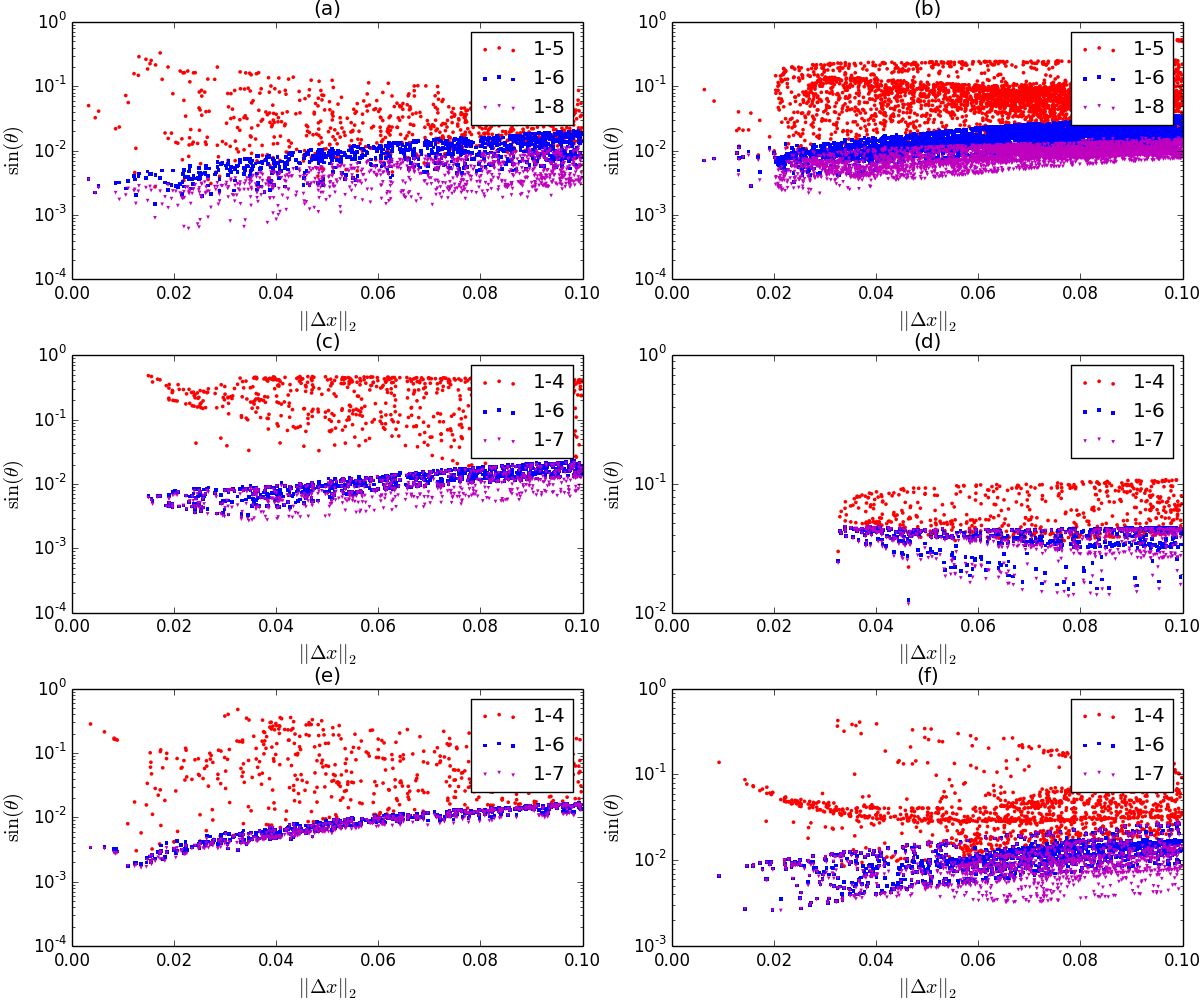
\includegraphics[width=1.0\textwidth]{ergodic_dis_angle2}
  \caption{
    The same experiment as \reffig{fig:ergodic_dis_angle_rpo1}.
    (a) (b) \cycle{rpo3} with {\Poincare} template point far away
    from slice border (left graph) and near the slice border
    (right graph).
    (c) (d) For \cycle{ppo2}.
    (e) (f) For \cycle{ppo9}
  }
  \label{fig:ergodic_dis_angle2}
\end{figure}

\begin{figure}[h]
  \centering
  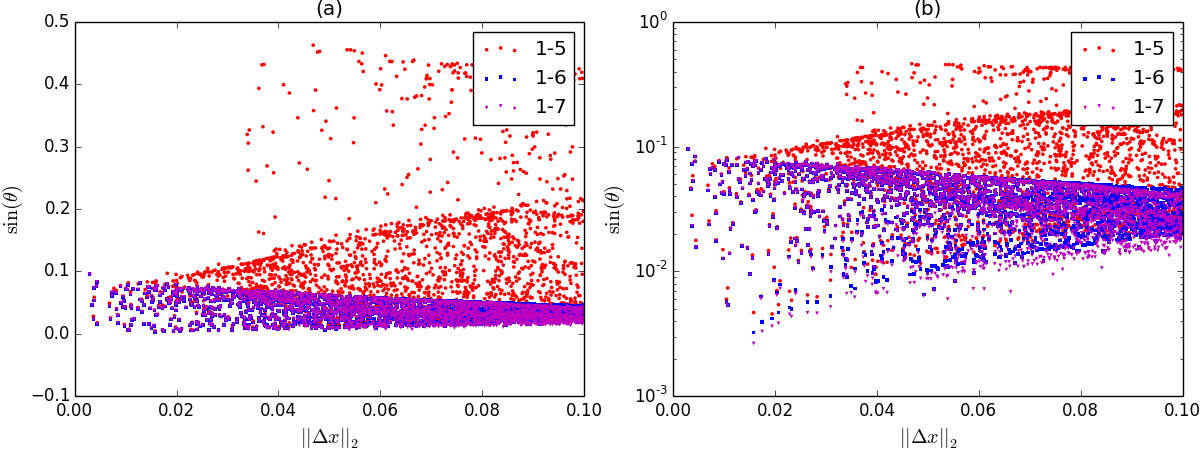
\includegraphics[width=1.0\textwidth]{ergodic_dis_angle_ppo4}
  \caption{
    The same experiment on \cycle{ppo4} as \reffig{fig:ergodic_dis_angle_rpo1} at the far side of slice border.
    (a) and (b) are the same
    experimental data with different schemes of y-axis scale.
   }
  \label{fig:ergodic_dis_angle_ppo4}
\end{figure}


\item[Predrag 2014-09-05]

Started taking notes from the WebEx meeting, cannot finish - someone
please take over with writing up the summary:

Hugues: do you get different plots if you separate statistics into
one real expanding eigenvector and the set of complex pair?

XD: there are very few orbits which are complex expanding pairs.
Expect similar statistics

Hugues: what is statistics of set of long orbits
(remove those shorter than - let's say 20)?

XD: will have a look

XD: blue and green curves are strictly bounded away from zero.

XD: we do not know why there are sharp peaks at larger angles?

PC: why is the green curve so different between \po s and \rpo s?

HC/KT: Has the peak in the blue curve physical meaning?

ES: is the peak in the blue (and red) curve at the same location for rpos and pos?

XD: Yes, almost the same location.

XD: I am worried about the results of \reffig{fig:ergodic_dis_angle_ppo4}.

HC: This ppo might be isolated from the attractor.

XD: However, the ergodic trajectory comes close to it.

ES: This has to do with how we measure distance. We always use Euclidean distance
but this cannot tell us if the orbit is on the attractor or not. We would neeed to
understand topology in order to answer this question, but this might be very hard.

ES: Maybe you could plot the intersection of the unstable manifold of
the orbit in \reffig{fig:ergodic_dis_angle_ppo4} with a {\PoincSec} and
the same for an ergodic orbit, and see if there is transverse distance
between them.

ES 2014-09-07: Also, at the points of closest approach of the trajectory and the ppo,
the velocities should not be misaligned if the latter is part of the attractor.

ES: (for next paper?) You could try to understand if the local dimension changes
along a long orbit that shadows two short orbits with different number of expanding
directions, \ie, produce a more sensible version of \reffig{fig:ks22shad} using
the smallest principal angle approach.

ES: {\PoincSec} is a bit confusing in 3D. Could you plot a 2D
projection, including points of intersection on the unstable manifold
of the rpo, rather than trajectories?

Everyone: We think there is now enough for a nice, short (max 4 pages) publication.
Kazz will produce the skeleton.

\item[Evangelos 2014-09-07] In order to understand what is going
on in \reffig{fig:ergodic_dis_angle_ppo4},
it might help to plot the data for the smallest principal angle for this orbit
and compare it to the data for a non-problematic orbit. There should be a difference
in how close the red curve comes to zero.

\item[Evangelos 2014-09-07] Actually \reffig{fig:ergodic_dis_angle_ppo4} might be
a way to tell if an orbit is part of the attractor or not.

\item[Xiong 2014-09-07] I tried to answer some of these questions.

\textbf{Blue and green curves are strictly bounded away from zero.}
this can be demonstrated by the y-log scale
\reffig{fig:statistic_angle_rpoppo_log}. Distribution $\rho(1/\theta)$
is not used here to show the boundedness because I did not get a good
exponential relation as
Kazumasa did in \refref{TaGiCh11}. One problem is panel (B):
the red line does not end on the y-axis. There is very small
gap. could we just account for it the shortage of data points?

\begin{figure}[h]
  \centering
  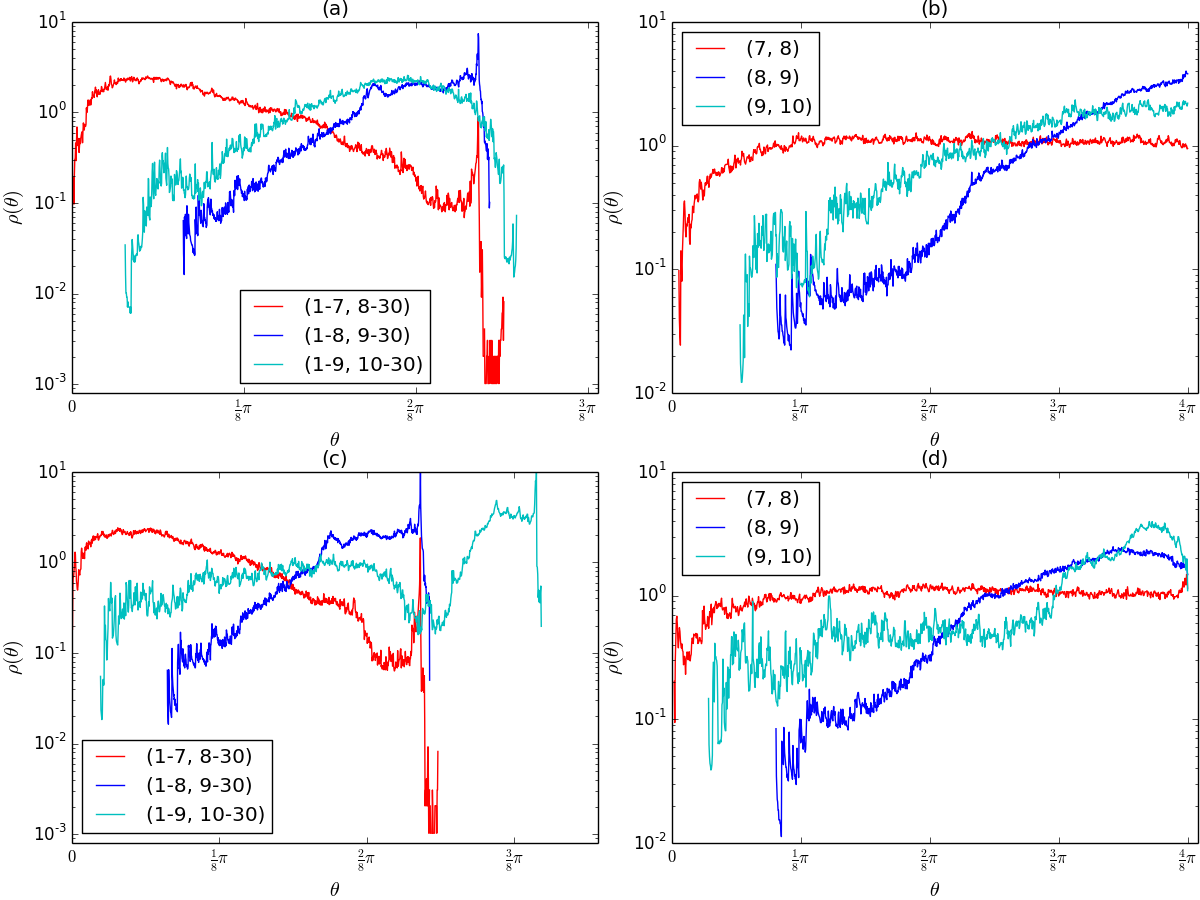
\includegraphics[width=1.0\textwidth]{statistic_angle_rpoppo_log}
  \caption{
  The same as in \reffig{fig:statistic_angle_rpoppo} but with log scale.}
  \label{fig:statistic_angle_rpoppo_log}
\end{figure}


\textbf{Do you get different plots if you separate statistics into
one real expanding eigenvector and the set of complex pair?} I presumed that
the orbits with two expanding directions (two real or complex conjugate)
are
far fewer than those with only one expanding direction; however it turns
out that I was wrong. Of the 240 pre-periodic orbits ($T<100$) and
239 relative periodic orbits, 167, respectively 159, have only
one expanding directions. So orbits with two expanding directions are about
one thirds of the total orbits with periods less than 100.
But the statistics
of these two types of orbits exhibit no striking difference as shown in
\reffig{fig:statistic_angle_rpoppo_AB}. Note that log scale is not used
because for curves oscillate strongly at the tails. Also number of bins in the
histogram \reffig{fig:statistic_angle_rpoppo_AB} is 400. For other figures,
1000 is used.
\begin{figure}[h]
  \centering
  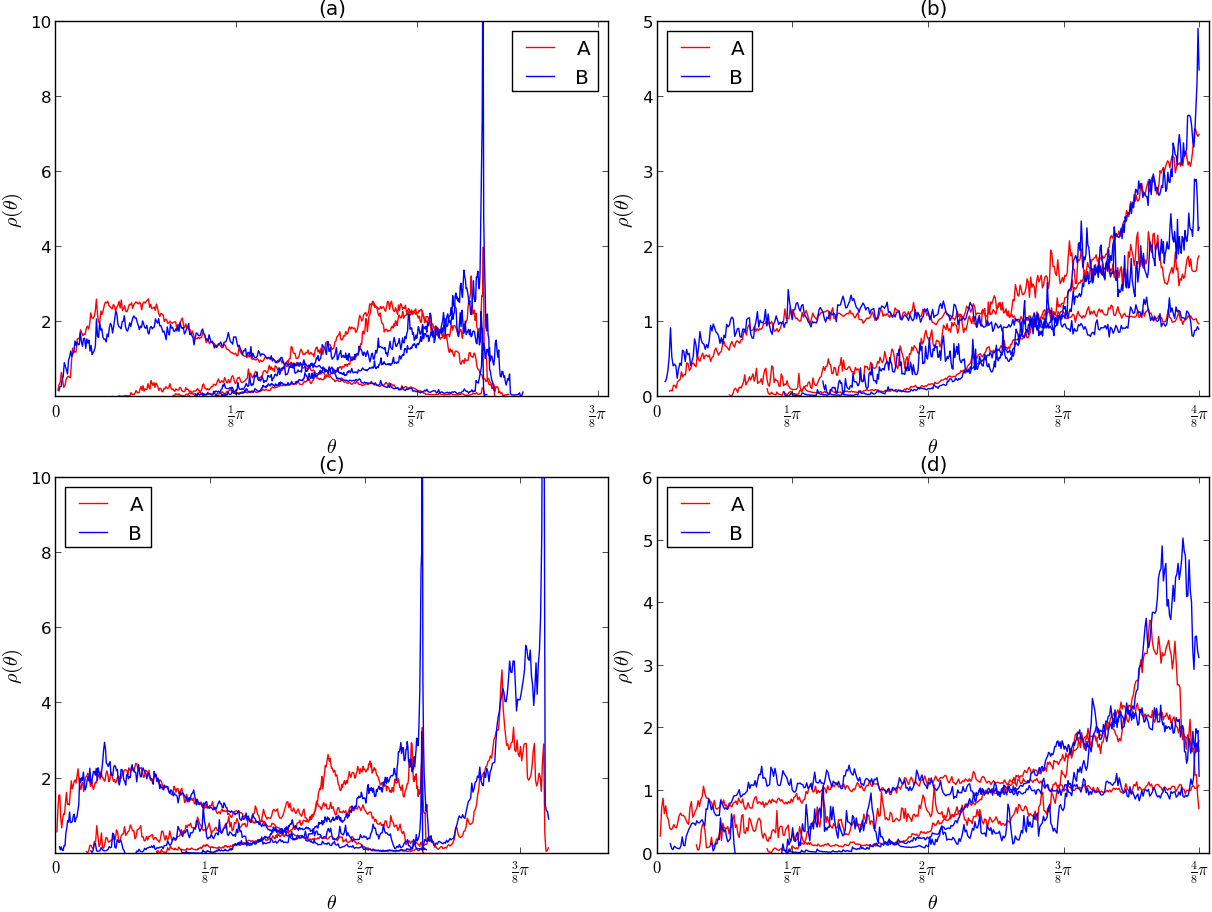
\includegraphics[width=1.0\textwidth]{statistic_angle_rpoppo_AB}
  \caption{Statistical result as in \reffig{fig:statistic_angle_rpoppo}
    with two types of orbits counted separately. Type A, B stand for the
    orbits with only one expanding directions and those with two expanding
    directions respectively. Each curve is normalized that the area under it
    is one.}
  \label{fig:statistic_angle_rpoppo_AB}
\end{figure}

\textbf{What is statistics of set of long orbits
(remove those shorter than - let's say 85)?}
Periodic orbits with $ 85 < T_p < 100$ are collected to give the
statistical result in \reffig{fig:statistic_angle_rpoppo_log_85}.
Again, there is no striking difference if only long orbits are taken
into consideration.
\begin{figure}[h]
  \centering
  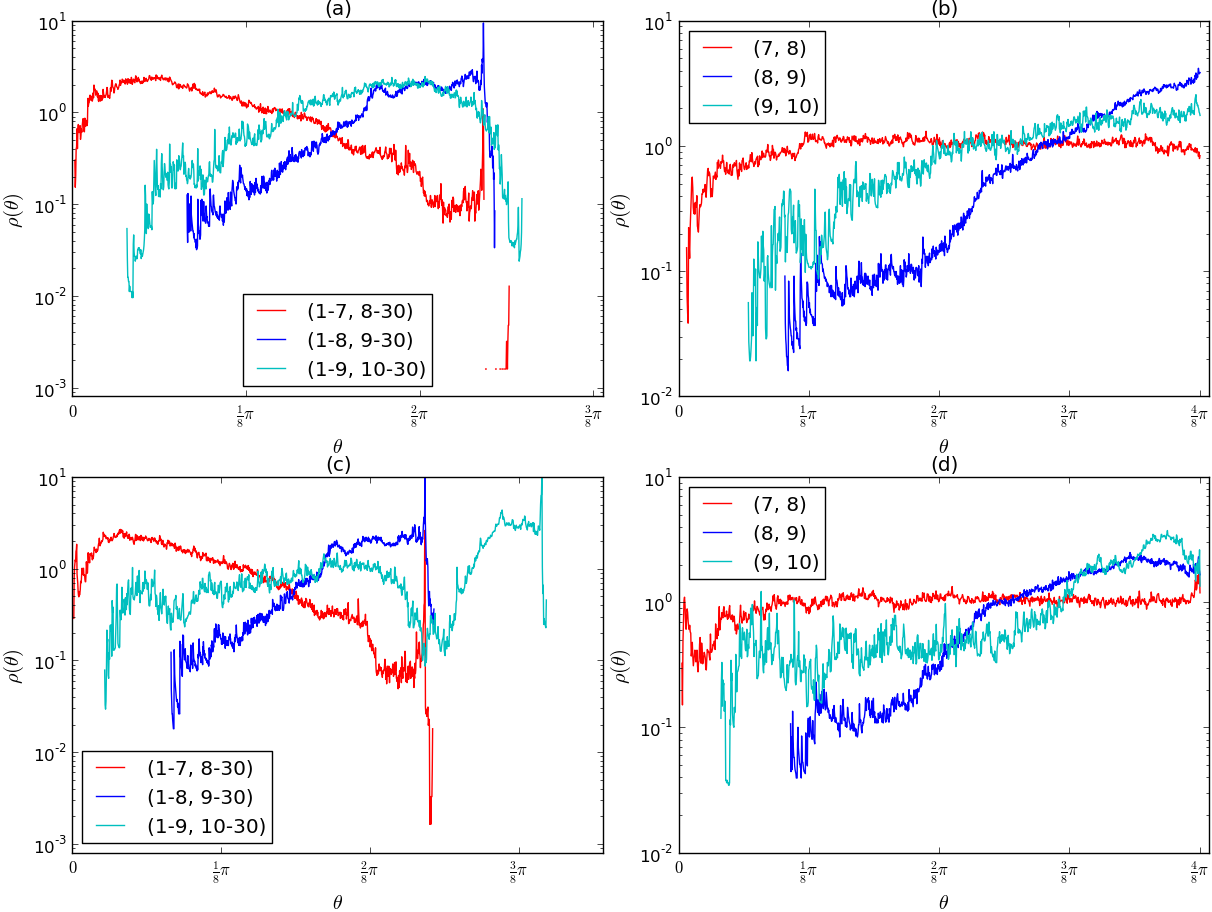
\includegraphics[width=1.0\textwidth]{statistic_angle_rpoppo_log_85}
  \caption{Similar to \reffig{fig:statistic_angle_rpoppo_log} but only count
  orbits whose period is larger than 85, that is, 131 out of 240 \cycle{ppo}s
  and 128 out of 239 \cycle{rpos}.
}
  \label{fig:statistic_angle_rpoppo_log_85}
\end{figure}

\textbf{why is the green curve so different between periodic orbits and relative periodic orbits?}
I am not sure, but I guess the reason lies on how we defined the subspace
spanned by the first 9 Floquet vectors. As I mentioned on the meeting,
if the 9th and 10th vectors form a complex conjugate pair, then both the
real part and the imaginary part will be counted to span the subspace.
For relative periodic orbits, the percentage of such orbits is 130/239, while
0\% for pre-periodic orbits; also, Floquet vectors with larger
index are more hyperbolicly disentangled from the physical mode. That is why
the angle between subspace (1-9) and (10-30) have a shift to large angle for
relative periodic orbits. On the contrary, for both \cycle{ppo} and \cycle{rpo},
the 8th Floquet vector never forms complex pair with the 9th one, so they
have similar distribution for angle between subspaces (1-8) and (9-30).

By the way, \cycle{rpo} is more prone to have complex conjugate Floquet vectors
than \cycle{ppo}. I think it is because the different definitions of Jacobian.
For \cycle{rpo}, $J_p = g_p J^{T_p}$. For \cycle{ppo}, $J_P = RJ^{T_p}$.
Here $g_p$ is a rotation, while $R$ denotes reflection.

\textbf{We do not know why there are sharp peaks at larger angles?}
From \reffig{fig:statistic_angle_rpoppo_AB}, we can see the peaks mainly
come from the orbits which have two expanding directions, but I still do not
know
why it should be like this. Also is this information very important?

\textbf{Maybe you could plot the intersection of the unstable manifold
of the orbit in \reffig{fig:ergodic_dis_angle_ppo4} with a {\PoincSec}
and the same for an ergodic orbit, and see if there is transverse
distance between them.} Pre-periodic orbit \cycle{ppo4} have two
expanding real directions with Floquet exponent 0.04 and 0.03
respectively. \refFig{fig:manifold_ppo4} gives its two dimensional
unstable manifold. following Chat\'{e}'s suggestion to look at the
local dimension at other points on this orbits, I found that I got
figure like \reffig{fig:ergodic_dis_angle_ppo4} on some points (black
dots in \reffig{fig:manifold_ppo4}); while some points on the orbit
(yellow dots in \reffig{fig:manifold_ppo4}) are capable to get the
local dimension. Does it mean that only part of \cycle{ppo4} is on the
attractor?

\refFig{fig:manifold_ppo4_m2} and \ref{fig:manifold_ppo4_m3} show how ergodic
trajectories intersect with {\PoincSec}. At least, we can identify two
different types of points I collected. I think that is why there are
two different structures
in \reffig{fig:ergodic_dis_angle_ppo4}. If \cycle{ppo4} has more than
one unstable bundle passing by the cluster, then we can say that the I am using
distance in a wrong way, but there is one unstable bundle penetrating the cluster,
so I still do not know why this template point fail to deduct information about
dimension. On the other hand, the 3d figures are just projections onto Fourier modes,
useful information may be lost.

\begin{figure}[h]
  \centering
  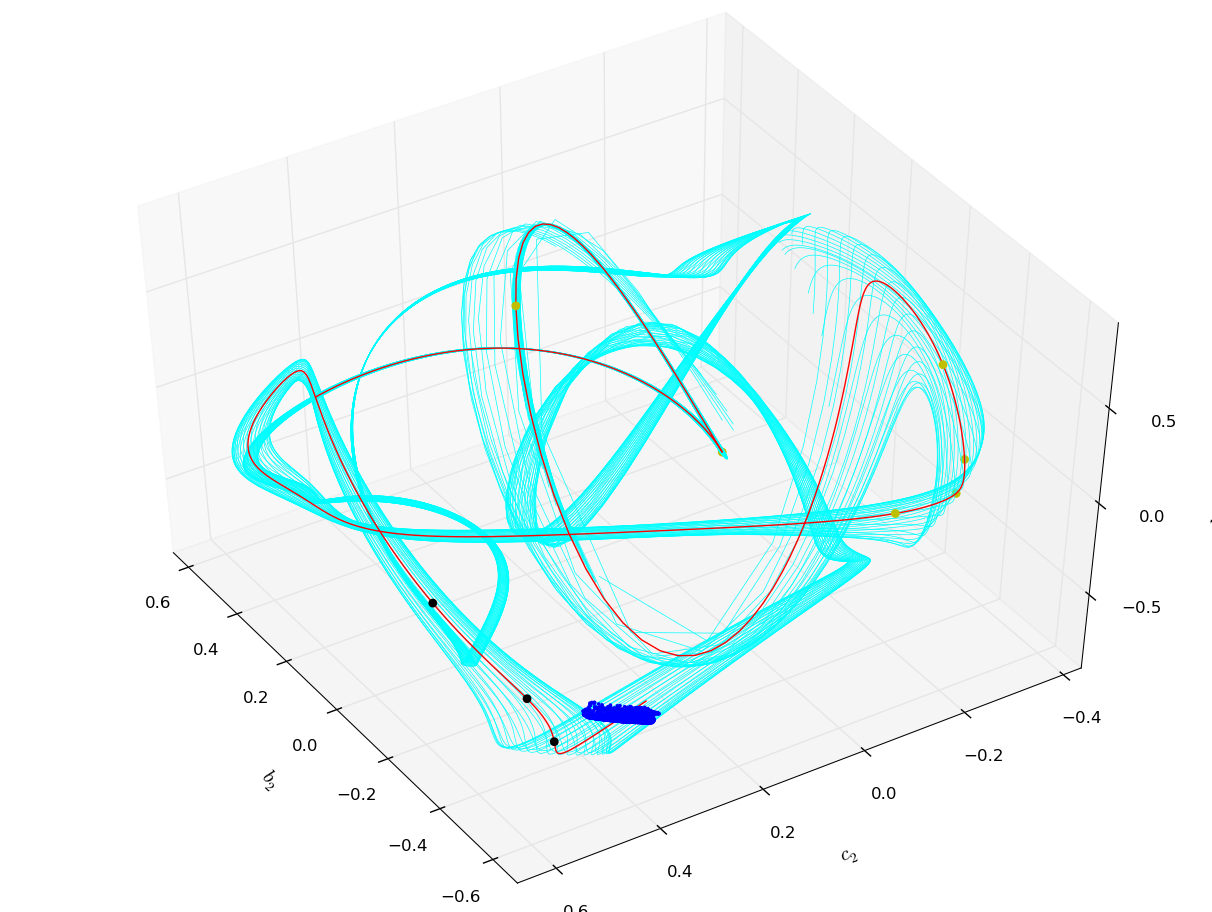
\includegraphics[width=1.0\textwidth]{manifold_ppo4}
  \caption{Unstatble manifold of \cycle{ppo4}. Red curve is the trajectory of
    \cycle{ppo4} for time $T_p = 33.38$. Black dots are the template points where I
    did not succeed to deduct information about local dimension; on the contrary,
    I did at yellow dots. The cluster of blue dots are the intersecting points between
    an ergodic trajectory and {\PoincSec} whose template point is the same as
    in \reffig{fig:ergodic_dis_angle_ppo4}. This figure is a projection onto the
    subspace of Fourier modes. x, y and z axes are $b_2$, $c_2$ and $b_3$ respectively.
  }
  \label{fig:manifold_ppo4}
\end{figure}

\begin{figure}[h]
  \centering
  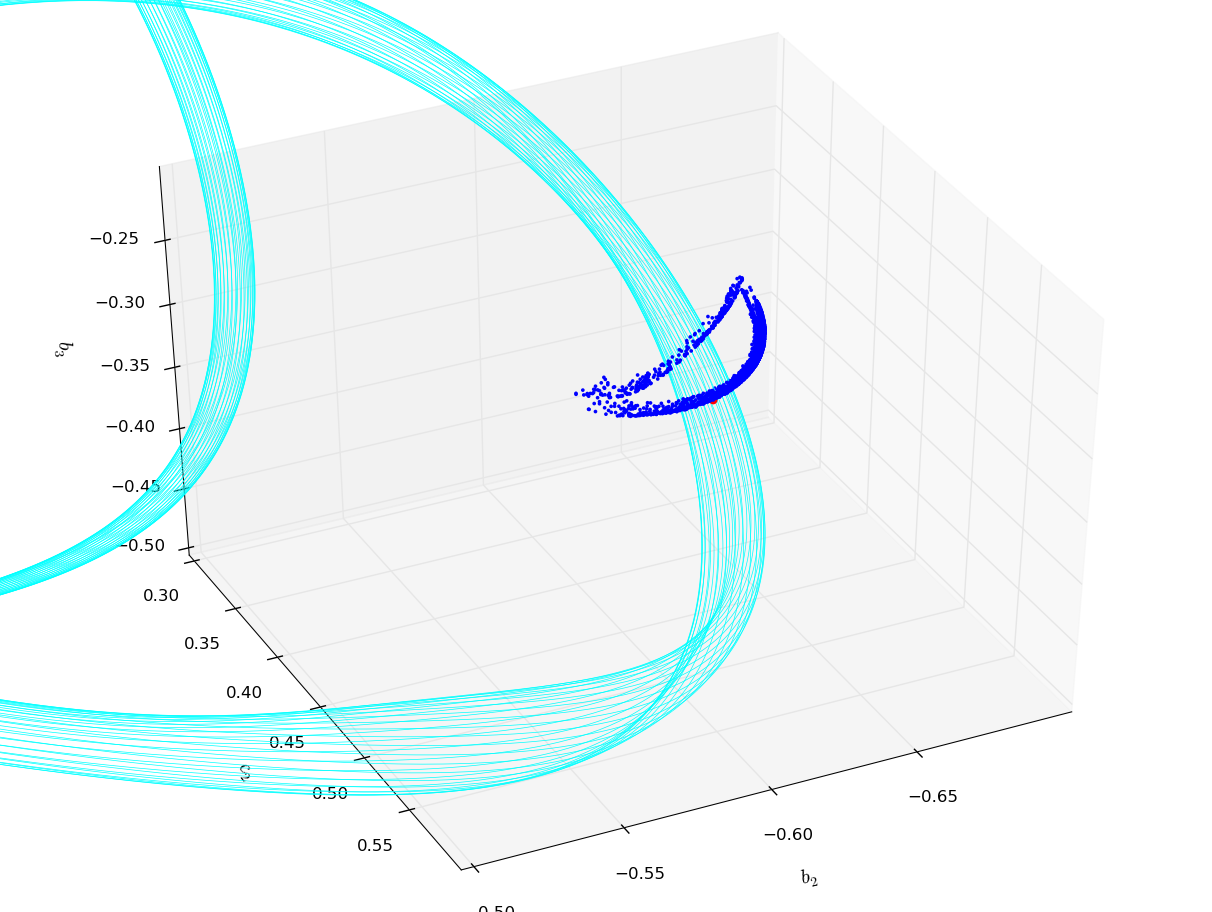
\includegraphics[width=1.0\textwidth]{manifold_ppo4_m2}
  \caption{The same as \reffig{fig:manifold_ppo4}. The part containing the cluster points
    are magnified. Red dot is the template point.
  }
  \label{fig:manifold_ppo4_m2}
\end{figure}

\begin{figure}[h]
  \centering
  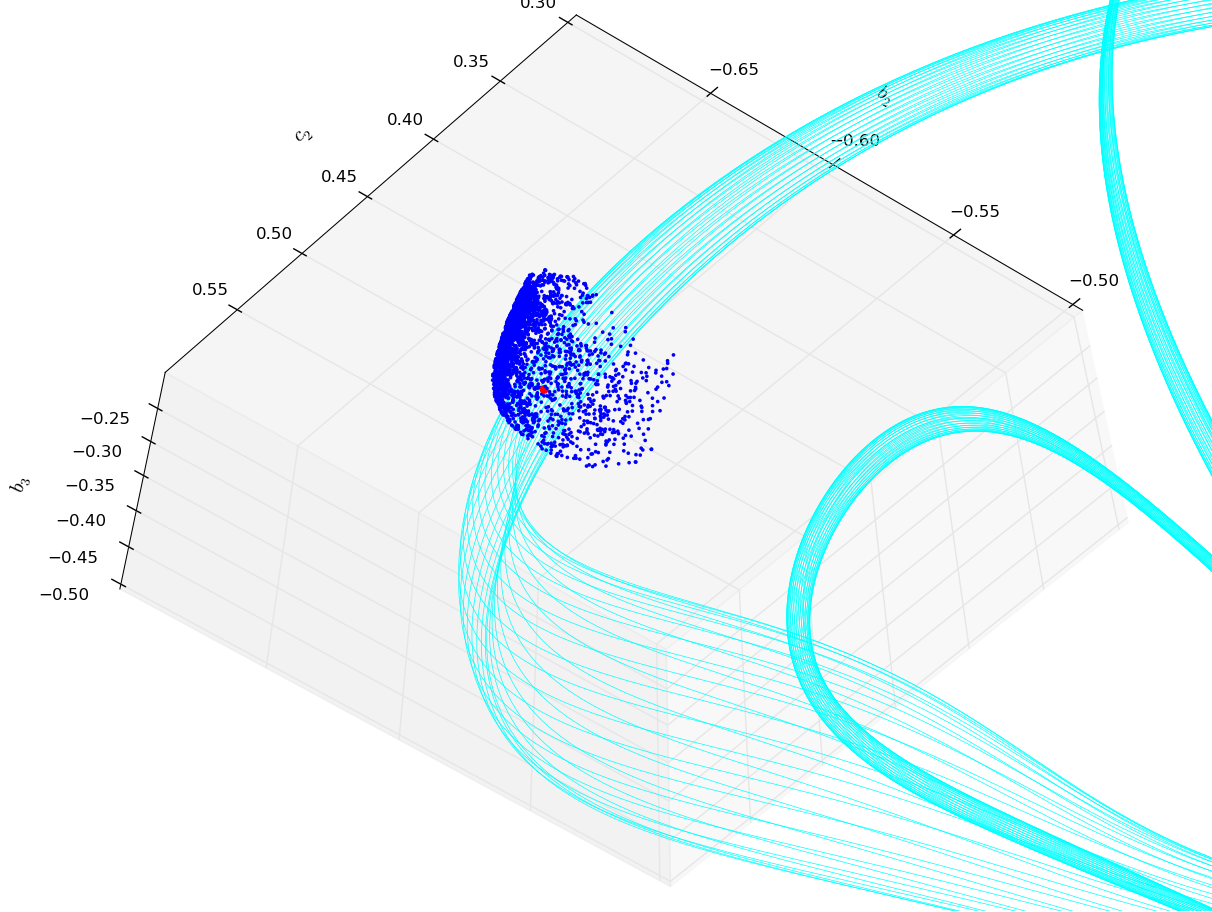
\includegraphics[width=1.0\textwidth]{manifold_ppo4_m3}
  \caption{The same with \reffig{fig:manifold_ppo4_m2} with a different angle.
  }
  \label{fig:manifold_ppo4_m3}
\end{figure}


\textbf{{\PoincSec} is a bit confusing in 3D. Could you plot a 2D projection?}
I am not sure whether 2d projection is better than 3d, and I tried 2d projection, It
does not seem more informative.

\item[2014-09-20 Evangelos] A brief summary of brainstorming session with Hugues and Xiong:

We think that \reffig{fig:ergodic_dis_angle_ppo4} is not as problematic as we initially thought.
The data points having small distance and large angle, presumably come from points that come close to
the ppo, but do not really shadow it. We suggested to Xiong to try to look only for points where the distance
is small and the ergodic trajectory stays close to the ppo for a while. Alternatively, he could test the
degree of alignment of the flow velocity at the close encounters. Basically apart from the condition
of distance being smaller than certain threshold, it might help to also impose the condition that the angle between
flow velocities is smaller than a threshold.

Regarding the data points with small distance and small angle for the red curve, we think that this is not
problematic. We understand this to mean that at certain points, tangent space can be spanned with fewer dimensions
than the 'attractor dimension.' We do not see a contradiction.

What worries us is that in some of the figures, e.g. \reffig{fig:ergodic_dis_angle_rpo1}, we see that as more
dimensions are taken into account the angle keeps getting smaller for what we think is the same point on the
trajectory. We believe that if the dimension of the attractor can be captured by the rpos, we should see an accumulation
towards a lower bound in angle. We suggest that Xiong adds more subspaces to these plots, to see if this happens.

If I understand this correctly, another way to state this, is that for a given point on the ergodic trajectory,
adding unphysical dimensions would lead to exponentially decreasing correction to the angle. Therefore it might help to
plot the correction in angle when you add an extra subspace, as a function of the number of included subspaces for a given point on a trajectory (a given difference vector).

Finally we think it might be worth looking at the variation of the smallest principal angle parametrized by time along a
rpo, for some rpos, both problematic and non-problematic.

\item[Xiong 2014-09-21] Some comments. \\
I updated \reffig{fig:ergodic_dis_angle_rpo1}. The original one is produced by
using the integrator in the 1st mode space; while all other figures are produced by
post-processing method. In order to keep the unitarity across all figures, I recollected
the intersection points for \cycle{rpo1} and found that \reffig{fig:ergodic_dis_angle_rpo1} only changes slightly. The original one is kept in the
svn repository.

\begin{figure}[h]
  \centering
  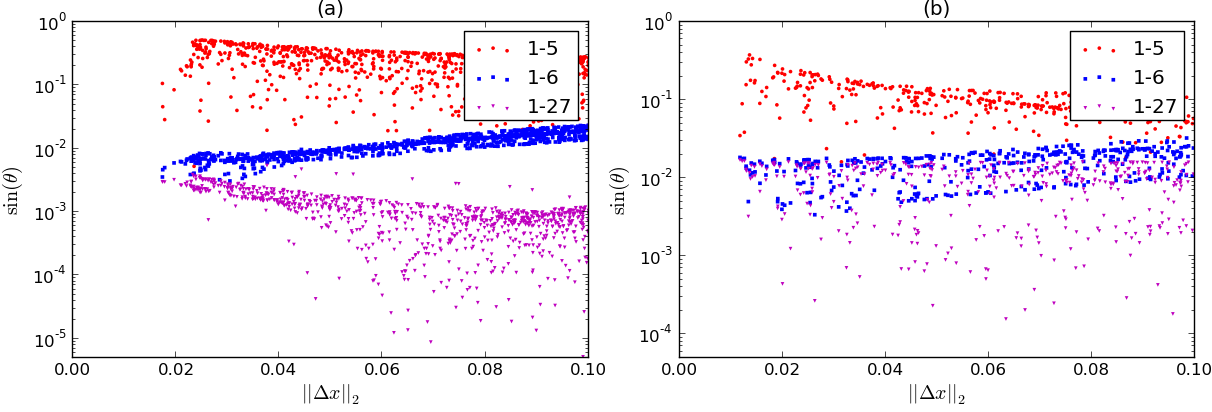
\includegraphics[width=1.0\textwidth]{ergodic_angle_rpo1_v2}
  \caption{The same as (b) (d) in \reffig{fig:ergodic_dis_angle_rpo1}
    except replacing $1-8$ by $1-27$.}
  \label{fig:ergodic_angle_rpo1_v2}
\end{figure}

\begin{figure}[h]
  \centering
  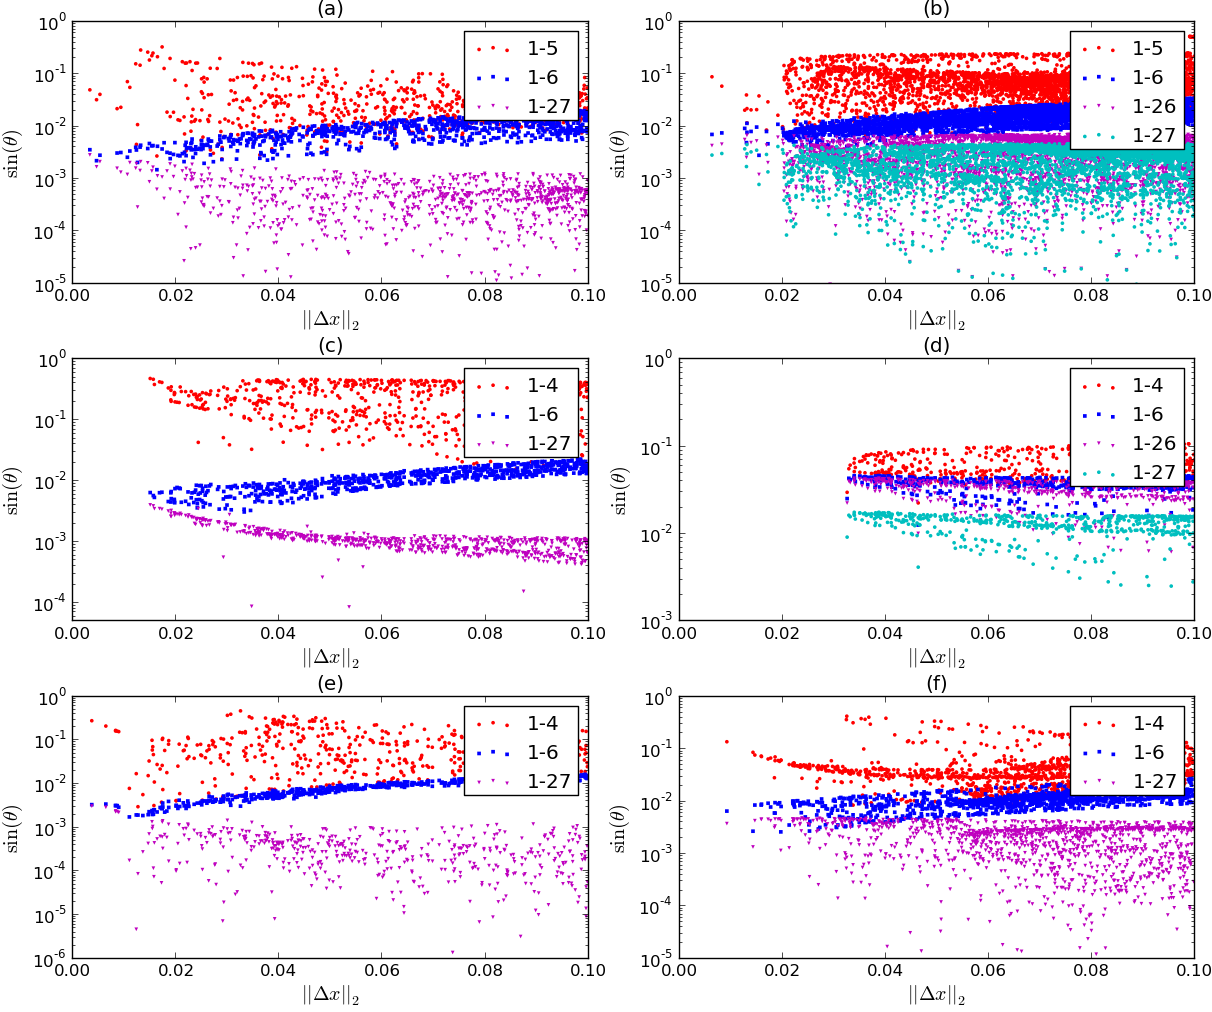
\includegraphics[width=1.0\textwidth]{ergodic_angle_collection}
  \caption{The same as \reffig{fig:ergodic_dis_angle2} except replacing case ($1-8$)
    by ($1-27$) or ($1-26$) .}
  \label{fig:ergodic_angle_collection}
\end{figure}

Dimensions are added to span the subspace when expanding the difference
vector. As shown in \reffig{fig:ergodic_angle_rpo1_v2}, angle tendency
for case ($1-27$) actually saturates with that for ($1-6$) when
difference vector decreases. The cases for other orbits are shown in
\reffig{fig:ergodic_angle_collection}. Note the dimension of this
system after slicing and {\PoincSec} is 28, so ($1-27$) refers to the
subspace spanned by all the Floquet vectors except the last one. As is
shown in these figures, the angle scattering points will indeed shift
down for large $||\Delta x||_2$ ($\gtrsim 0.04$), but they converges to
the case $(1-6)$ when these points get closer to the template point.
Looking at these figures makes me feel better about
\reffig{fig:ergodic_dis_angle_ppo4}. At the same time, we should be
aware of panel (b) (d) in \reffig{fig:ergodic_angle_collection}. It
seems that ($1-26$) saturate to ($1-6$) but not for ($1-27$) at these
two template points.

To investigate the velocity alignment between {\Poincare} intersecting points and
the template
points, \reffig{fig:velAngDistributionCollection} shows the angle distribution
for each template point in different orbits. Although \cycle{ppo4} has relatively large
portion in large angles $0.25$, it looks normal since \cycle{rpo3} also
behaves similarly. The other three cases have maximal angle around $0.16$. Also I tried
to exclude the intersecting points which are misaligned (velocity angle $\theta > 0.16$),
the result is similar to \reffig{fig:ergodic_dis_angle_ppo4}. Another way I tried to get rid
of the velocity misalignment is just recording even closer recurrence points. For all the
above experiments, the threshold of accepting a {\Poincare} intersecting point is that
the difference vector should have Euclidean length less than 0.1, but now I tried a
smaller threshold 0.02. The result is shown in \reffig{fig:ergodic_angle_ppo4_002}.
In this case, the velocities at {\Poincare} intersecting points are well aligned with
the velocity at the template points ($\theta < 0.07$). It is clear that 5 Floquet vectors
at this point are not enough to span the local space, and $(1-4)$, $(1-27)$ produce the
similar result.  But the figure is not sharp enough. It seems that smaller threshold is
required to see the tendency.

\begin{figure}[h]
  \centering
  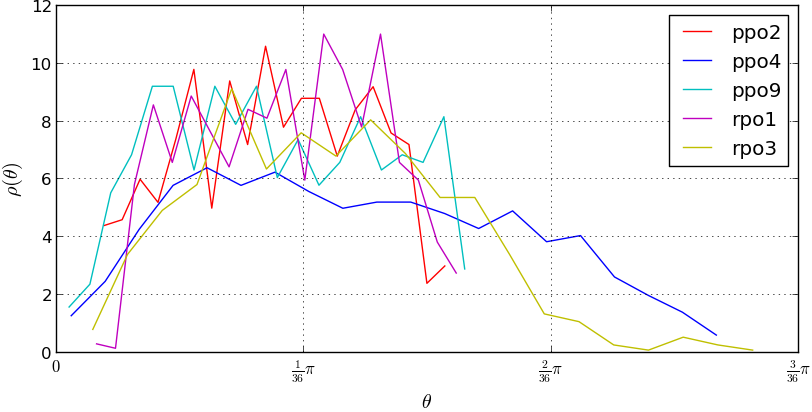
\includegraphics[width=1.0\textwidth]{velAngDistributionCollection}
  \caption{ Distribution of the angle between the velocities at the {\Poincare} intersecting
    points and the template point for different orbits. The template point is the farthest
    away from the slice border. 20 bins are used in this histogram plot and the area under
    each line is normalized. Sorry about the previous histogram plots, they are normalized
    incorrectly, and I will update them in future. But they will not change too much.
    }
  \label{fig:velAngDistributionCollection}
\end{figure}

\begin{figure}[h]
  \centering
  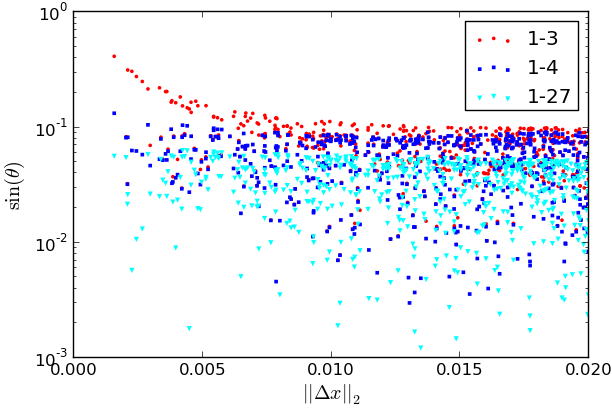
\includegraphics[width=0.7\textwidth]{ergodic_angle_ppo4_002}
  \caption{The same as \reffig{fig:ergodic_dis_angle_ppo4} but with closer
    intersecting points. 588 points were collected in a whole day. Note, here
    (1-3) (1-4) are used.
    }
  \label{fig:ergodic_angle_ppo4_002}
\end{figure}

\refFig{fig:hyperbolicitySample} shows how angle changes along the
three different orbits.

\begin{figure}[h]
  \centering
  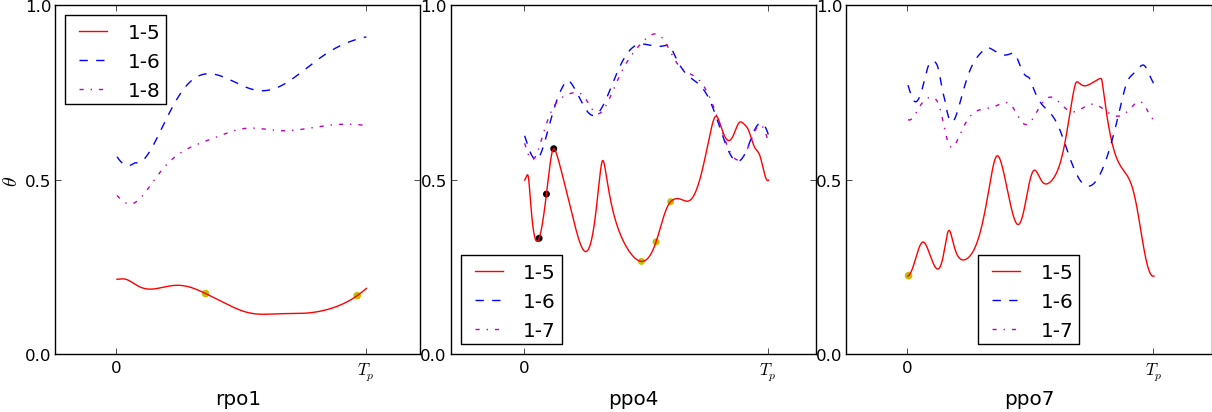
\includegraphics[width=1.0\textwidth]{hyperbolicitySample}
  \caption{The smallest principal angle between the subspace
    spanned by the Floquet vectors indicated by the legend and the one spanned
    by the remaining Floquet vectors. Three different orbits are used here.
    Yellow dots donate the non-problematic points;  black dots donate the
    problematic points.
    }
  \label{fig:hyperbolicitySample}
\end{figure}

\item[2014-09-23 Kazz to Xiong and everyone]
I enjoyed the updates. Here are my comments, suggestions, and questions.
A skeleton of the paper follows.

\textbf{Distribution of principal angles.}
The results in \reffig{fig:statistic_angle_rpoppo_log}
(log-scale plot of \reffig{fig:statistic_angle_rpoppo}) are nice,
 but not enough to claim that the blue and turquoise distributions are bounded
 away from zero.
It's true you don't have data for $\theta$ close to zero,
 but if you extrapolate, I would say the distributions decrease exponentially
 with $\theta$ (look straight in \reffig{fig:statistic_angle_rpoppo_log})
 and reach non-zero densities at $\theta = 0$,
 so the physical and unphysical subspaces are not strictly split.
To claim that these distributions are bounded, data must be fitted with
 a function that is bounded or has an essential singularity at $\theta =0$
 (e.g., $\rho(\theta) \sim \exp(-\text{const.}/\theta)$).
You say ``Distribution $\rho(1/\theta)$ is not used here
to show the boundedness because I did not get a good exponential relation'',
 but how bad was it?
How difficult is it to accumulate more statistics
 so that the tail of the pdfs extends by, say, one more digit?
As these will be the central results of the paper,
 I am most concerned with this problem.

\textbf{Angle vs distance plots.}
As I mentioned in the web discussion,
 if a given subspace covers the physical subspace,
 one would expect a linear relationship between the angle and the distance,
 as shown in \refref{TaCh11}.
This is because, in this case,
 the only reason the difference vector is not in the subspace
 is that the physical manifold deviates from its linear approximation
 as the distance increases.
If we assume that the manifold is smooth
 (as should be if it corresponds to the inertial manifold),
 the deviation from the linear approximation is
 in the order of $||\Delta r||_2^2$ in distance,
 so, in angle, $||\Delta r||_2^2 / ||\Delta r||_2 = ||\Delta r||_2$.
Therefore, I suggest to plot \reffig{fig:ergodic_dis_angle_rpo1}
 and similar figures in loglog scales, and compare the slope with -1.

\textbf{Concerning \reffig{fig:ergodic_dis_angle_ppo4}.}
I agree with what is written in the brief survey of the brainstorming session.
It is particularly important to understand why the blue and purple dots
 do not approach zero as the distance decreases.
It would be perfect if this is caused by ergodic trajectories that come nearby
 but not shadow the orbit (I found this very interesting), but the result
 in \reffig{fig:velAngDistributionCollection} doesn't seem to be convincing.
I have an alternative suggestion:
 you can decompose the difference vector
 using the bases given by the Floquet vectors,
 and see how each component grows/shrinks with time.
If the trajectory is topologically close to the orbit,
 each component should grow or shrink at the corresponding Floquet exponent.
One may use it as a criterion
 to distinguish topologically close orbits and others.
Of course, to check this idea,
 one should compare problematic and non-problematic orbits along this line
 and see if the above speculation is correct.

\textbf{rpo vs ppo?}
It seems that the ensemble of rpos and that of ppos
 produce essentially the same result (\reffig{fig:statistic_angle_rpoppo_log}),
 which is very nice.
But then, what do you think is the role of rpos?


\textbf{Provisional structure of the paper.}
Assuming that all above pending problems will be resolved,
 here is what I propose for the structure of the paper.

\begin{enumerate}

\item Introduction
\begin{itemize}
\item Introduce the periodic orbit expansion of chaos.
Describe how powerful it is (e.g., to compute dynamical averages),
 and more importantly, how conceptually important it is
 (orbits form the skeleton of chaos).
Stress however that it is unclear to what extent this picture is valid
 for spatially extended systems
 (briefly mention what is known and what is missing).
\item Explain main results in \refref{YaTaGiChRa08,TaGiCh11}
 (decoupling of the physical/spurious subspaces).
This approach seems to be well suited for the periodic orbit description,
 because all the necessary quantities (Lyapunov exponents/vectors)
 can be defined for the orbits as well,
 in terms of the Floquet exponents and vectors.
However, applying the same method to an orbit makes no sense,
 because the length of an orbit is finite,
 so the angle distribution of any pair of vectors is bounded.
One should look at an ensemble of orbits!
\end{itemize}

\item Methods
\begin{itemize}
\item system, numerical integration, algorithm to find orbits,
 algorithm to compute Floquet exponents/vectors and their precision
 (precision is important because usually it's difficult to obtain
 strongly contracting Floquet modes).
\end{itemize}

\item Main results
\begin{itemize}

\item Figure 1: Visualize how an ergodic trajectory approaches an orbit.
Figure like \reffig{fig:xdpo1ppo191} between an ergodic trajectory and an orbit
 is good enough. Showing how the Euclidean distance evolves is even better
 (like Fig.2b in \refref{TaCh11}).

\item Figure 2: Display a figure like \reffig{fig:statistic_angle_rpoppo_log}.
We need a clear figure (so clear data and/or analysis) to show that
the distribution becomes bounded as soon as the subspace includes
 a certain number of Floquet vectors.
Compare this number with the physical dimension
 estimated from the ergodic trajectories
 (which is nine, including three neutral modes; see Fig.4a in \refref{TaCh11}).

\item Figure 3: Display a figure like \reffig{fig:ergodic_dis_angle_rpo1}
 or \reffig{fig:ergodic_dis_angle2}, which shows that each orbit carries
 information of the physical dimension
 (we however need to use ergodic trajectories here;
 to construct the physical dimension purely from orbits,
 one needs an ensemble).
However, we first need to understand \reffig{fig:ergodic_dis_angle_ppo4}.

\item It would be wonderful
 if we find an orbit indicating a smaller physical dimension
 (as the brainstorming session discussed
 about \reffig{fig:ergodic_dis_angle_ppo4}, but without strange behavior
 of the blue/purple dots).
Try to find such an orbit, and if you do so, look for anything particular
 about this orbit (in particular, hyperbolicity).
If we succeed in doing this, we can discuss relation
 to the dimension variability (see, e.g., \refref{KaGrPrLaSi02}).
This will significantly increase the impact of the paper,
 because this is something that we cannot do solely with ergodic trajectories
 (at least at present).
\end{itemize}

\item Conclusion.
\end{enumerate}

Any comments and suggestions are welcome, of course!
\begin{figure}[h]
  \centering
  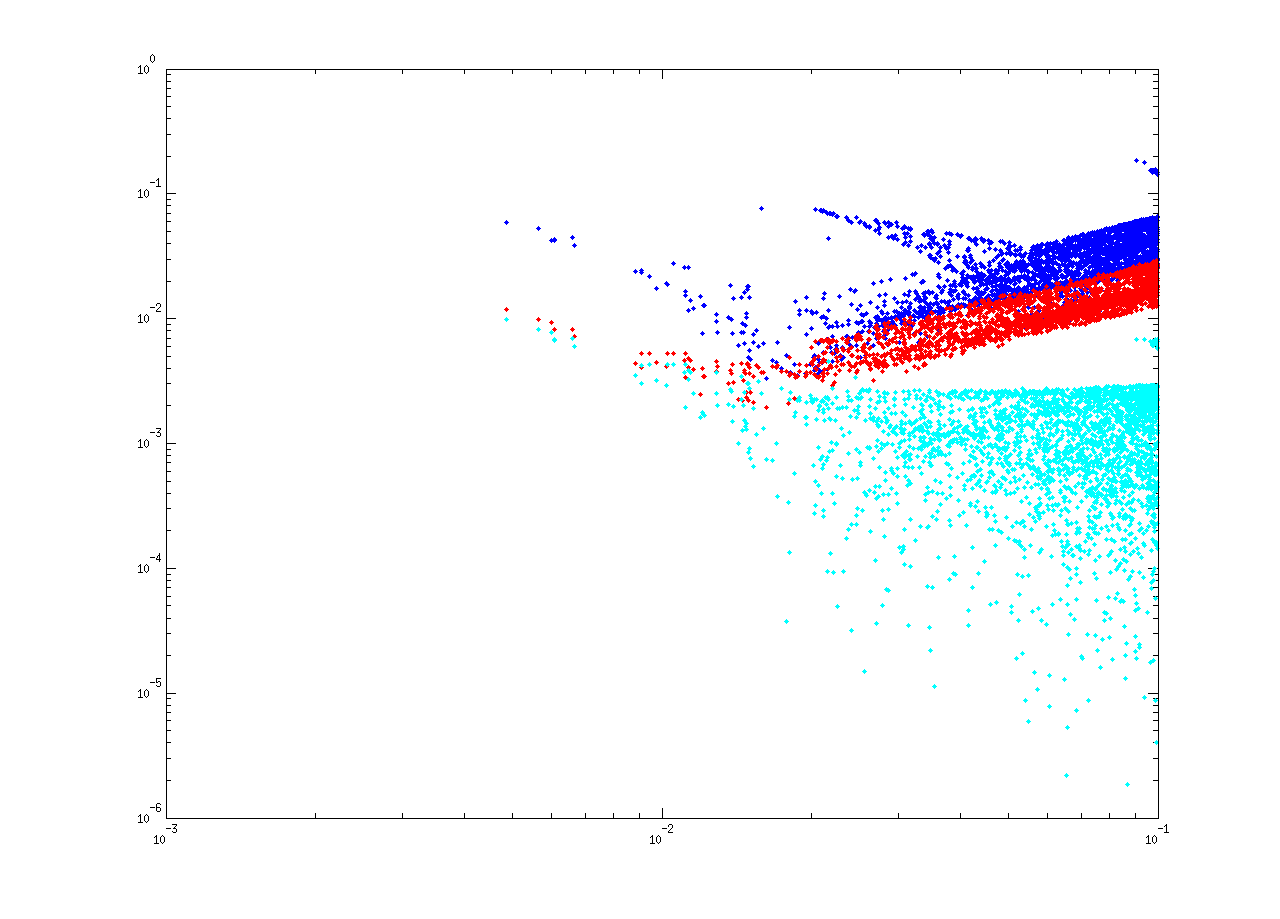
\includegraphics[width=1.0\textwidth]{ergodic_angle_ppo1}
  \caption{The same experiment as in
  \reffig{fig:ergodic_angle_ppo4_002} conducted on \cycle{ppo1}. The
  blue, red and green points refers to subspace (1-5), (1-6)
  and (1-27) respectively. 2864 points are recorded.
}
  \label{fig:ergodic_angle_ppo1}
\end{figure}

\item[Xiong 2014-10-10]
  I am not sure what I understand about angle distributions is
  correct or not.

  \textbf{dominated splitting} was invented as a relaxed version of
  hyperbolicity since the latter is a very strong property or restriction.
  According to\rf{Enrique03}, an f-invariant set
  $\Lambda$ is said to have dominated splitting if the tangent bundle can
  be decomposed into two continuous invariant subbundles
  $T_\Lambda M = E \oplus F$, such that:
  \[
  ||Df^{n}_{/E(x)}||\cdot||Df^{-n}_{/F(f^n(x))}|| \le C\lambda^n \,,\quad
  \text{for all} \quad x\in\Lambda\,, n\ge 0
  \]
  with $C>0$ and $0<\lambda<1$. In my view, it is
  $||J^n(u)||/||J^n(v)||\le C\lambda^n$ for $u\in E$ and $v\in F$.
  Basically, it means that the expanding rate in subspace $F$ is larger
  than the expanding rate in the subspace $E$ at every instant point along
  the trajectory. This definition leads to the boundedness of angle
  between these two subspaces $\angle (E, F)$. Let $\lambda'=C\lambda$, then
  \[
  ||Ju|| \le \lambda' ||Jv|| = \lambda'(||J(v-u)||+||Ju||)
  \]
  so
  \[
  ||v-u|| \ge \frac{1-\lambda}{\lambda}\frac{||Ju||}{||J||}
  \]
  Here, you can regard the matrix norm as the vector induced Euclidean
  norm $||A||=\max(||Ax||_2/||x||_2)$, therefore the angle between these
  two subspaces is bounded away from zero.

  Jairo points out (proposition 3.1 in\rf{Bochi05} or proposition 2.3
  in\rf{Bochi04}) that if the dominated splitting is not satisfied at
  point $y$, then there exists an $(\epsilon_0,\kappa)$-realizable sequence
  ${L_0, \cdots, L_{m-1}}$ at y such that
  \[
  L_{m-1}\cdots\L_0(v) = \omega
  \,,
  \]
  where $v\in E$ and $\omega\in J^{m}(F)$. I am sorry I could not fully
  understand this proposition, but it seems that if the dominated
  spitting is not satisfied, then there is possibility that vectors in
  one subspace can evolve into another subspace at sometime, which means
  these two subspaces may get entangled at some point along the trajectory.

  What confused me is the physical picture of tangency (angle be zero).
  If tangency happens, it means that the set of covariant vectors are not
  linearly independent, so they does not span the whole tangent space.
  The only possibility I could get up with is that Jacobian matrix $J_p$
  does not have a whole set of Floquet vectors. Just like matrix
  $\bigl(\begin{smallmatrix}
    1&1\\ 0&1
  \end{smallmatrix} \bigr)$
  has only one eigenvector:
  $\bigl(\begin{smallmatrix}
    1\\ 0
  \end{smallmatrix} \bigr)$.
  The periodic eigendecomposition will give you two same eigenvectors then.
  However, numerically, these two eigenvectors can not be exactly same.
  What do you think ?

  Pavel V.Kuptsov uses principle angles to investigate the hyperbolicity
  of a chaotic system. In \refref{Kuptsov12}, Fig.1 is very similar to our
  result \reffig{fig:statistic_angle_rpoppo_log}. Since \KS\ system is not
  hyperbolic, we are actually testing dominated splitting, but the idea is the
  same. Also if we QR and LQ decompose the eigenvector matrix $v=Q_1R=LQ_2$ and
  define $P=Q_1^\top Q_2$, then, as Pavel points out,
  submatrix $P(1:k,1:k)$ is singular, which is in accordance with my picture.

  I think I will try to investigate the dominated splitting of these \cycle{rpo}
  and \cycle{ppo}.
%Also I am still working on the problems left from last meeting. but the
%progress is very slow. I am sorry about it.

  \begin{table}[h]
    \centering
    \begin{tabular}{c  c | c c}
      E & $\rho$ & E & $\rho$  \\ \hline
      1-1  &     0.487   &   1-9  &           0 \\
      1-2  &     0.336   &   1-10  &          0 \\
      1-3  &     0.178   &   1-11  &          0 \\
      1-4  &     0.059   &   1-12  &          0 \\
      1-5  &     0.029   &   $\cdots$ & 0       \\
      1-6  &     0.017   &   1-28  &          0 \\
      1-7  &     0.008   &   1-29  &          0 \\
      1-8  &     0       &         &            \\
       \\
       \\
       \\
       \\
         \\
       \\
       \\
    \end{tabular}
    \caption{Percentage of violence of dominated splitting for
      \cycle{rpo} and \cycle{ppo} whose period is less than 100.
      The zeros in the table are exact. $E$ is the subspace spanned
      by the indexed Floquet vectors.
    }
    \label{tab:dominated_splitting}
  \end{table}

\item[2014-11-26 Xiong Ding]

I conducted a series of new experiments in order to resolve the
problems proposed by the last meeting. First, I use part of periodic
orbits with $ 100 < T < 120$ to collect the angle distribution as
previous did in \reffig{fig:statistic_angle_rpoppo}. I find that the
distribution is rather stable. Second, I give up {\PoincSec} and turn
to use human labor to inspect each approaching incidence in
\reffig{fig:ergodic_angle_rpo1_v2} to locate the true shadowing part
approximately. In this way, I obtained a better angle-distance
scattering plot \reffig{fig:disAngScatter_ppo4}.
\begin{figure}[h]
  \centering
  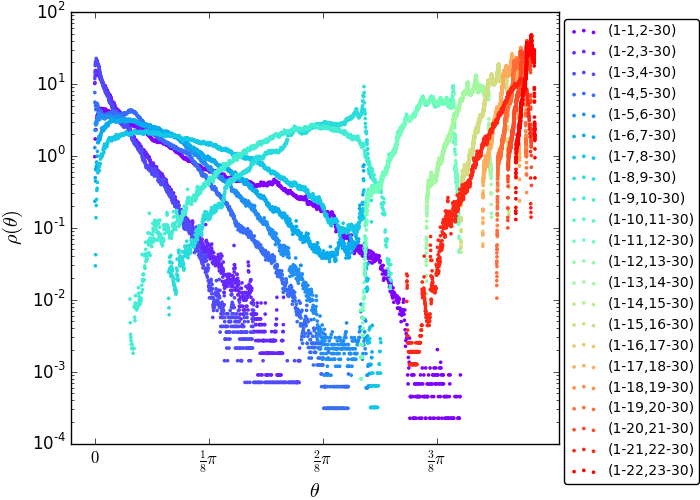
\includegraphics[width=0.48\textwidth]{angle120ppoSpace1} \hfill
  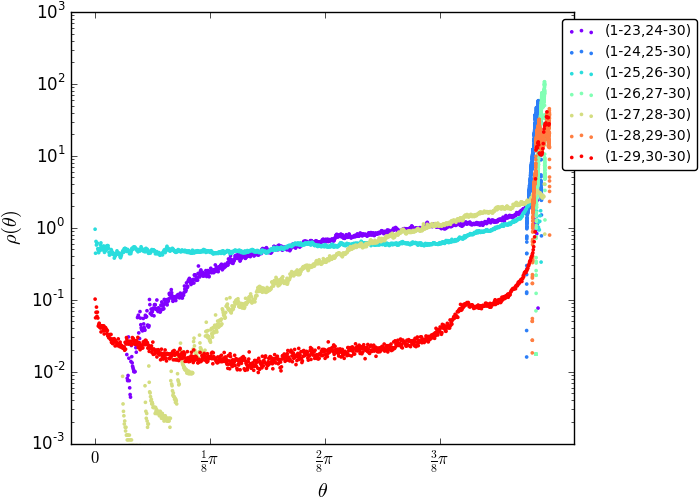
\includegraphics[width=0.48\textwidth]{angle120ppoSpace2}
  \caption{Angle distribution $\rho(\theta)$ versus $\theta$
    for \cycle{ppo} which has $ T < 120$.
    Left: angle distribution for subspace indexed up to 22.
    Right: angle distribution for subspace from 23 to 29.
  }
  \label{fig:angDist_ppo}
\end{figure}
\begin{figure}[h]
  \centering
  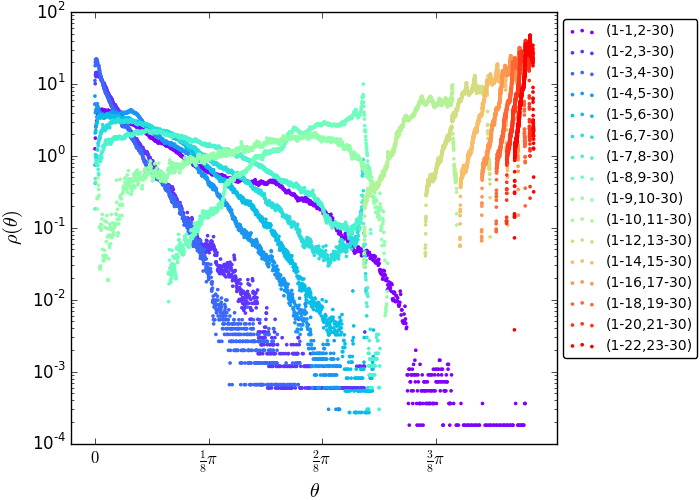
\includegraphics[width=0.48\textwidth]{angle120rpoSpace1} \hfill
  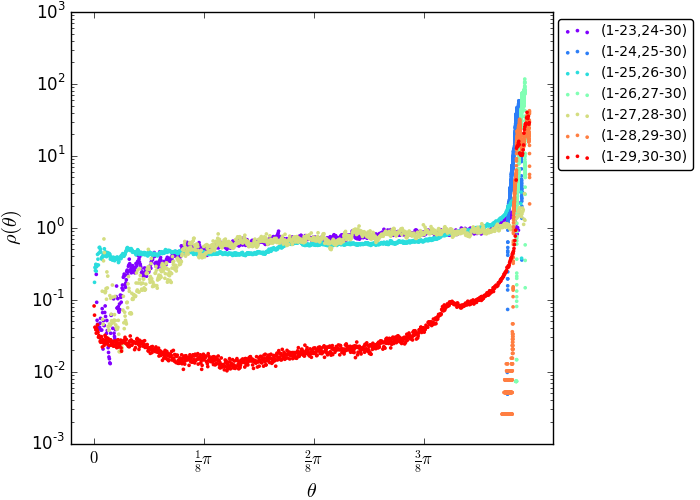
\includegraphics[width=0.48\textwidth]{angle120rpoSpace2}
  \caption{The same as \reffig{fig:angDist_ppo}, but for \cycle{rpo}s.
  Note that subspace cut at 11, 13, 15, 17, 19, 21 are not plotted
  because the sample points are very few. For example, the 16th, 17th
  Floquet vectors form a complex pair
  for all \cycle{rpo}s, so the collected
  data for (1-16,17-30) is zero.}
  \label{fig:angDist_rpo}
\end{figure}
\begin{figure}[h]
  \centering
  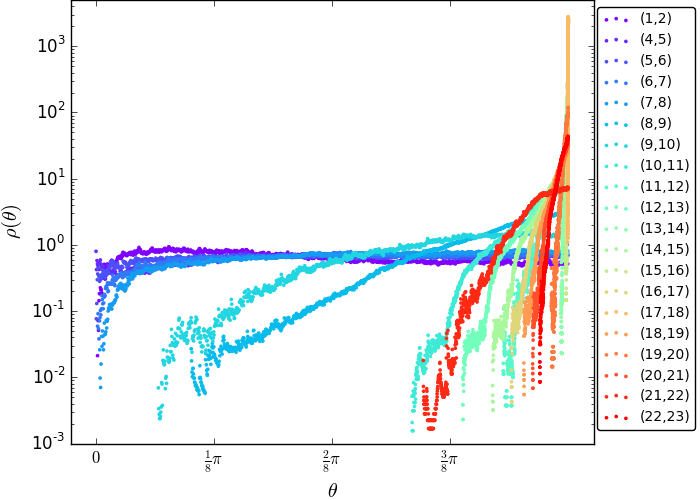
\includegraphics[width=0.48\textwidth]{angle120ppoVector1} \hfill
  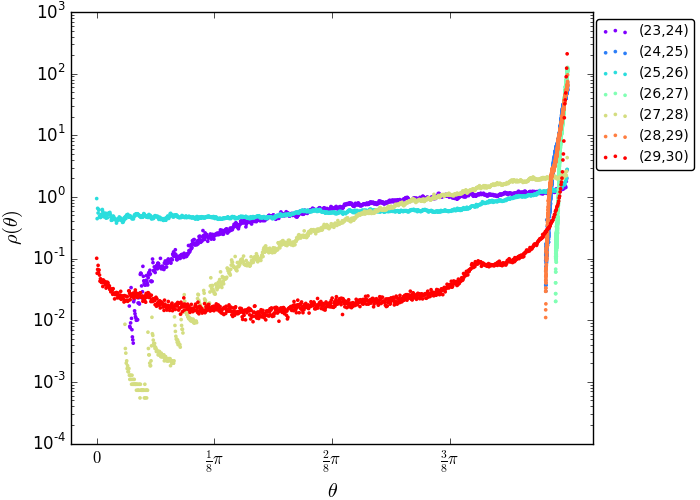
\includegraphics[width=0.48\textwidth]{angle120ppoVector2}
  \caption{ Angle distribution for Floquet vectors with adjacent
    indices for \cycle{ppo}.
  }
  \label{fig:angDistVec_ppo}
\end{figure}
\begin{figure}[h]
  \centering
  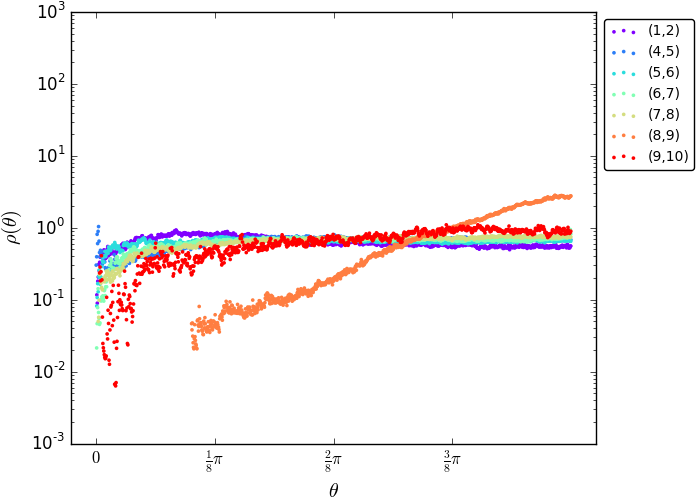
\includegraphics[width=0.48\textwidth]{angle120rpoVector1} \hfill
  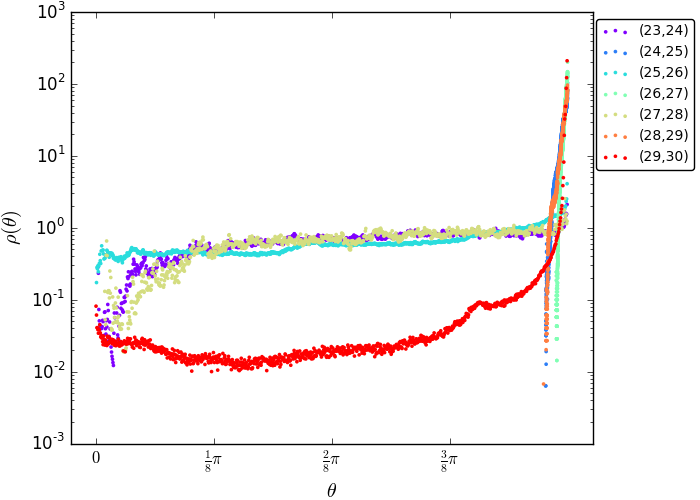
\includegraphics[width=0.48\textwidth]{angle120rpoVector2}
  \caption{The same as \reffig{fig:angDistVec_ppo} but for \cycle{rpo}.
  Note a lot of cases are omitted because either Floquet vector is
  complex.
}
  \label{fig:angDistVec_rpo}
\end{figure}

In \reffig{fig:angDist_ppo}
, angles between subspaces spanned by
Floquet vectors are collected for \cycle{ppo}, \cycle{rpo} with
period $ 100 < T < 120$, in contrast to the previous experiments
with $T < 100$.
\Xiong
{2014-11-27}
{Not all of the orbits with $100 < T < 120$ are used. For some
of them, my multishooting routine fails to refined them because some
of the long orbits converge to short orbits. Only 85 percent of them
are used to do the statistical experiments. Even though, the number
of orbits considered here is much more than the orbits with $T < 100$.}
Several points need to be mentioned.
First, we observe that the angle distribution is
rather stable. Data collected from $T < 100$ with that
collected with $100 < T < 120$ has similar shape. For instance,
\reffig{fig:angDist_ppo} is very close to
\reffig{fig:statistic_angle_rpoppo_log_85}. This means that this
distribution is a result of the geometrical structure of the
inertial manifold of this system (although the relation is unknown
until we find the symbolic dynamics).
It demonstrates that  short periodic orbits consist
of the skeleton of an ergodic system, and, in future,
studying only the fundamental POs is enough  to get the physical dimension of
a system. Second, \cycle{ppo}s and \cycle{rpo}s are still treated
separately because I find that the angle distribution for 8th and 9th Floquet
vectors is zero for \cycle{ppo} but not for \cycle{rpo}
\reffig{fig:angDistVec_ppo} and \reffig{fig:angDistVec_rpo}.
I guess the difference is related to the different definition of Jacobian
for \cycle{ppo} and \cycle{rpo}. For rpo, a rotation matrix is multiplied
to Jacobian, and it mix the real and complex component of Fourier modes.
So in \reffig{fig:angDist_rpo}, angle distribution of (1-10) vs (11-30) is
plotted other than (1-9) vs (11-30). On the other hand, no matter whether
there is tangency between 9 and 10, these two directions are both
contracting, their tangency would not change the local dimension.

\begin{figure}[h]
  \centering
  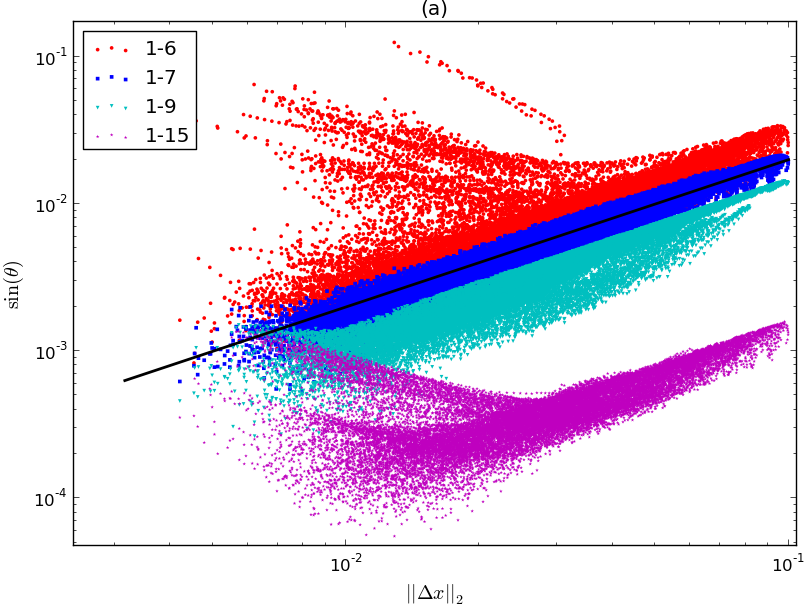
\includegraphics[width=0.8\textwidth]{disAngScatter_ppo4}
  \caption{Angle distribution versus length of difference vector for
    \cycle{ppo4}. Each point
    is an experimental incidence. Since we are on the slice, (1-6) corresponds
    (1-7) in the full state space. There are total 22592 shadowing points in
    this graph coming from collecting 700 ``V'' shapes.
  }
  \label{fig:disAngScatter_ppo4}
\end{figure}

\begin{figure}[h]
  \centering
  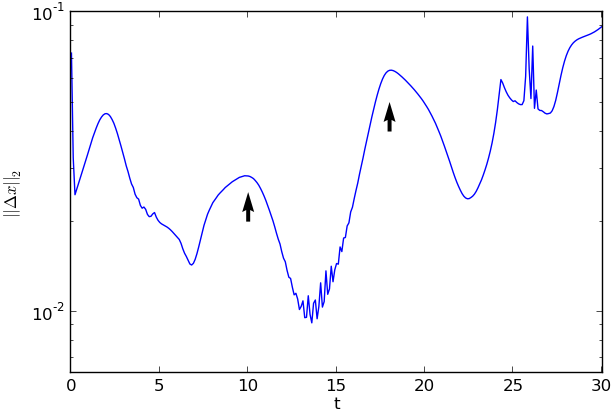
\includegraphics[width=0.48\textwidth]{disStructure_ppo4}
  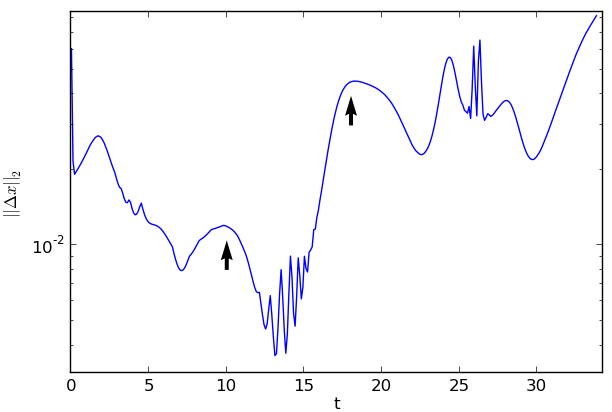
\includegraphics[width=0.48\textwidth]{disStructure_ppo4_2}
  \caption{Two shadowing examples. Y axis is Euclidean length of
    difference vector. X axis is time.}
  \label{fig:disStructure}
\end{figure}

\begin{figure}[h]
  \centering
  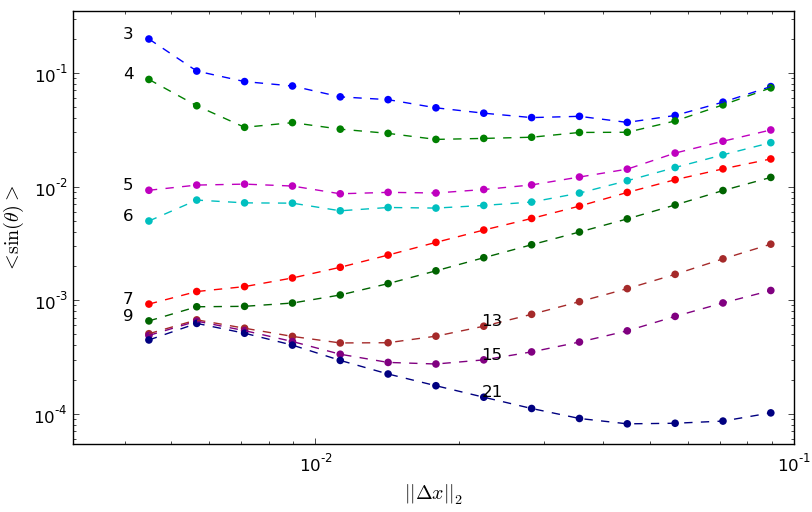
\includegraphics[width=0.8\textwidth]{disAngAverage_ppo4}
  \caption{Averaged version of \reffig{fig:disAngScatter_ppo4}.}
  \label{fig:disAngAverage_ppo4}
\end{figure}

Also, I gave up the idea of {\PoincSec} when testing the relation
between angle distribution and length of difference vector. So only
slice is used to reduce the dimension by one, and Floquet vectors are
projected to the slice. Previously, we have a lot of substructures in
the $\sin(\theta)$ versus $||\Delta x||_2$ plot, but now, as shown in
\reffig{fig:disAngScatter_ppo4}, the substructures are gone. Also, the
concern that the angle-distance plot may  saturate for small difference
vector is not a problem, because data for distance as small as
$10^{-2.6}$ does not show any flatting tendency.

Figure \ref{fig:disAngScatter_ppo4} also shows that \cycle{ppo4}
is not problem any more, as contrast to used to be.
The problem is that when collecting data, we should make sure
that the ergodic orbit is indeed shadowing the PO, not just passing around.
This is difficult in numerical simulation since the unstable manifold of POs
are folding around the orbit.
Small Euclidean distance does not suffice to indicate
shadowing because small Euclidean ball around
one point along the Po may contain several
layers of unstable manifold. To resolve this problem, I take the procedure
as follows. First, we define a threshold trapping time $\tau_0$
and only collect approaching incidences which are trapped by the Po
for at least $\tau_0$. This will
substantially reduce the fake shadowing incidences. Second, although, the
ergodic segment found in the first step is trapped for a long time, it does
not mean that the whole segment is really shadowing the Po. It is highly
possible that only a part of the segment is, but the other part has crossed
the  unstable manifold and land on another layer of it.  So, in this step, we
need to observe the distance - time plot \reffig{fig:disStructure}
to find the real shadowing part. This is done by a graduate student's nude
eyes.

The V shape in \reffig{fig:disStructure} enclosed by two arrows
is the true shadowing incidence. An ergodic trajectories is attracted
by Po in the first part, and is pushed away by the Po in the second part.
There is a slight oscillation in the middle
valley because the ergodic point switches between stable manifold and unstable
manifold there. At the same time, it is hard for an ergodic orbit
to follow the stable manifold for a long time, as opposed to following
unstable manifold. As a consequence, there is a large percentage
of broken ``V'' shape (\reffig{fig:disStructure}(b)) in approaching incidence
profile, and in this case, we only record the points on the right segment.
Those V shapes with no oscillating valley are not recorded because I doubt
they are not switching between stable/unstable manifolds, but at the ridge
of a stable/unstable manifold witch has a shape curvature.

When choosing threshold trapping time $\tau_0$, smaller one will give us
more shadowing incidences; while, larger one will result in closer
approach. I tried a few different $\tau_0$s, I can only get approach as close
as $10^{-3}$.

Figure \ref{fig:disAngAverage_ppo4} gives the averaged angle distributions.
For (1-i) with $i < 7$, the angle density blows up or gets flattened as
$||\Delta x||$ decreases. (1-7) is almost a straight line with slope 1, but
the left most part has a small fluctuation. for (1-i) with $i>7$, they first
decrease as distance decreases, but at some point, they all saturate to
(1-7). This is reasonable, because when distance is large, omitting the last
few Floquet vectors does not have a large influence on angle. Note that, the
power spectrum of difference vectors almost concentrate on the first few
modes; while, when distance is large, the first 7 Floquet vectors are good
enough to expand the difference vector, so they saturate to (1-7).

\item[2014-12-08 Evangelos] I just had a look at the data for RPO$_4$. Period is
$T=33.4$, there two unstable directions with multipliers $\Lambda_1=4.4$, $\Lambda_2=-3.5$
and all other multipliers are real (I hope Xiong could verify this). Now I am a bit
confused as to where the oscillations in \reffig{fig:disStructure} come from,
since there are no complex multiplier pairs.

\item[2014-12-10 Hugues] In \reffig{fig:angDist_ppo} and \reffig{fig:angDist_rpo}:
these figures should be redone with all orbits (both "short" and "long").
importantly for each orbit, one should pay attention to "degeneracies" intheir
Floquet spectrum. I.e.: if the dimension of the manifold we want to consider falls
"in between" a degenerate subspace formed by a pair of Floquet eigenvalues, then
this orbit should not be included for that dimension. Also, we would like to see
this figure with more subspace dimensions than those currently shown, in particular
larger dimensions than the largest shown, in order to see whether the distribution
of angles goes away from zero as the dimension is increased. Also info about smaller
dimensions than the smallest shown could be intersting. All this for our internal
use, not necessarily to include in a paper.

\item[2014-12-10 Hugues] In \reffig{fig:disAngScatter_ppo4}:
How does it split if one considers only the down-going part of the Vs (and the
up-going parts)? What deos it look like if one only uses the local minima of the
time series of the distance, irrespective of that distance. This has the advantage
of exploring much smaller distances than those probed by the manual selection
method, and, very importantly, it does not require any manual intervention.

If plotting local minima gives some "satisfactory" answer, then similar figures
should be built using other orbits, including the short ppo1 orbit used by Kazz
before.

Then again, how would such a figure look like for an orbit which is "almost
non-hyperbolic", i.e. those orbits participating to the small-angle tail in fig.42?
could we see that the magic dimension is changed?


\item[2014-12-10 Hugues]
How about generating upo for a case with fixed boundary conditions, large enough to
be of significantly different dimension than the one treated so far? and then re-do
the whole thing... this is just to annoy Predrag...!


\item[2014-12-10 Xiong to Evangelos, Hugues]
I use \cycle{ppo4} because the previous results about this
orbit is terrible \ref{fig:ergodic_dis_angle_ppo4}. The
largest two Floquet multipliers are indeed 4.4 and -3.5,
but I find that the slops of `V' shapes vary and do not
follow these two numbers. I assume that this is because
we are measuring Euclidean norm not the distance along the
(un)stable manifold. For the oscillation, initially, I
just attribute it to the switching process between stable and unstable
manifolds, and presume that this process is accomplished
not immediately but in a few steps, so oscillation happens.
Now it is clear  that this explanation is not satisfactory,
I will look closer at this approaching incidence. By the way,
\cycle{ppo1} and \cycle{rpo1} also have such oscillation when
distance gets smaller than $10^{-2}$.

I will rerun my code to generate data following Hugues' advice.
It may take two or three days (I am preparing for a final exam these
two days:)). Thanks very much for writing down these requirements.
But when dealing with different boundary conditions,
this task may take more than a few days.
I do not know whether there is existing repository
documenting these \po s for this new setting.
In my side, it almost requires me to rewrite
the code of integrator and try to find a few hundred \po s
before conducting any experiments.

I will work tomorrow. Thanks.

\item[2014-12-12 Evangelos to Xiong] There are two things that I could think
these oscillations might tell us: 1) We are not in the linear
neighborhood of the PO (otherwise everything would be controlled by
{\stabmat} eigenvalues), 2) Below some distance between orbits, you reach
the limits of spatial resolution, so you cannot really distinguish
between the PO and neighborhing orbits.

I can see from Ruslan's database that this particular orbit was very
frequently detected, so I would guess that it must leave in the attractor
and we should be able to reach its linear neighborhood. Option (2) is more
likely since we know that refining the orbits by doubling the number of
modes changes the period to third significant digit. So you might want to
try the same computation with twice as many modes.

\item[2014-12-12 Xiong to Envangelos]
  If the modes are doubled, the initial condition has changed by 3 digits,
  but does it means that they are just slightly
  different points in the same orbit but not that more modes increase
  resolution dramatically?

\item[2014-12-12 Xiong]
  Figure \ref{fig:angDist_ppo} \ref{fig:angDistVec_ppo},
  \ref{fig:angDistVec_rpo} and \ref{fig:angDist_rpo} are updated with
  more subspace cases. Also $T<100$ and $100<T<120$ are combined.
  At right panels, angle extended to zero for subspace cut at
  odd indices. I guess it is because the time step I am using (h=0.02) is
  too large to separate the two modes which correspond to two nearly
  degenerate Floquet exponents for large indices.
  I remember once Kaza told me he used much
  smaller time step in his simulation. Anyway, the left panels are
  pretty convincing. Need I decrease the time step and
  redo all computation? That means a lot of coding.

\item[2014-12-15 Xiong]
  \refFig{fig:disAngScatter_ppo4} is updated in
  \refFig{fig:disAngScatter_localMin} with only points with minimal
  distance. The distribution diverges as distance decreases.
  \begin{figure}[h]
    \centering
    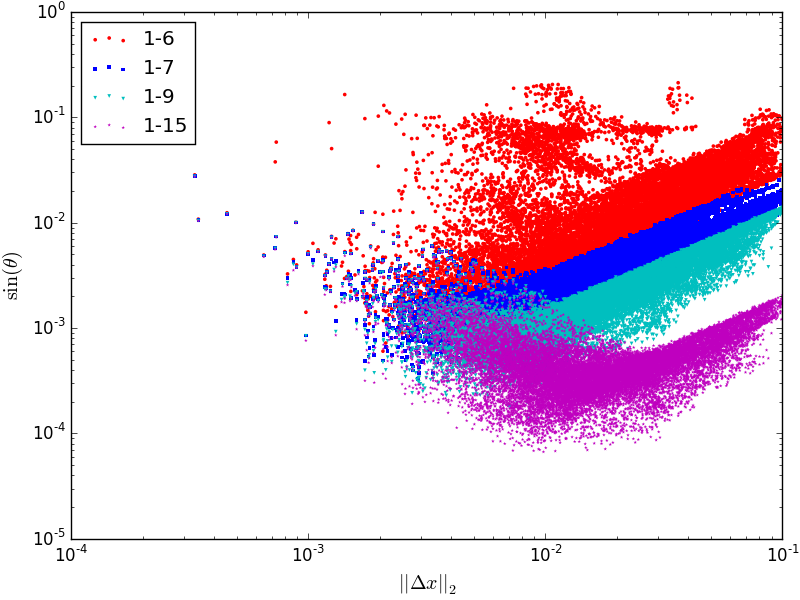
\includegraphics[width=0.48\textwidth]{disAngScatter_ppo4_localMin}\hfill
    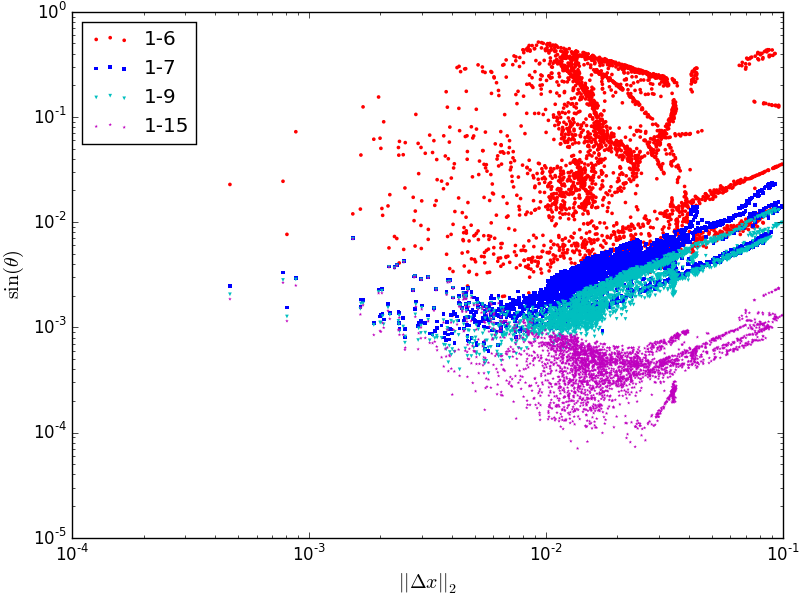
\includegraphics[width=0.48\textwidth]{disAngScatter_rpo1_localMin}
    \caption{Left: for \cycle{ppo4}.
      The same with \reffig{fig:disAngScatter_ppo4} but only
      the local minimal point in each shadowing incidence is recorded. Right:
      for \cycle{rpo1}.}
    \label{fig:disAngScatter_localMin}
  \end{figure}


\item[2014-2-11 Xiong]
I tried to double the number of Fourier modes to integrate the system and
for Floquet vectors calculation.The new plots are generated in
\reffig{fig:disAngScatterN32_1} and \reffig{fig:disAngScatterN32_2}.

 \begin{figure}[h]
    \centering
    (a)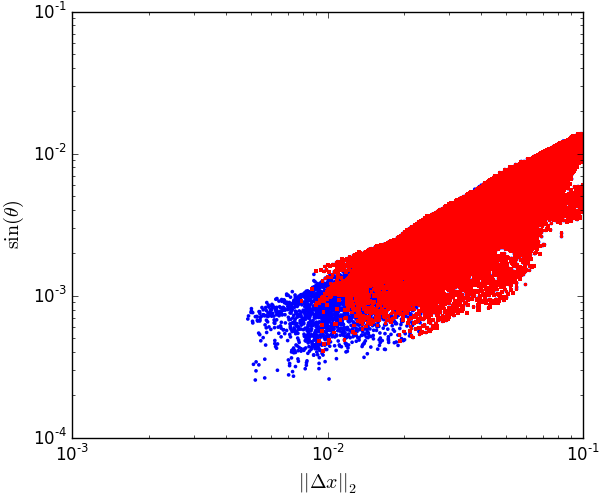
\includegraphics[width=0.45\textwidth]{disAngScatter_ppo1x10}\hfill
    (b)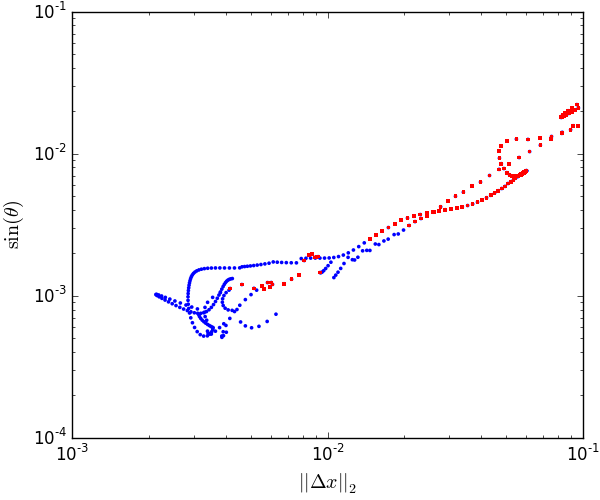
\includegraphics[width=0.45\textwidth]{disAngScatter_ppo2x10sT30}
    (c)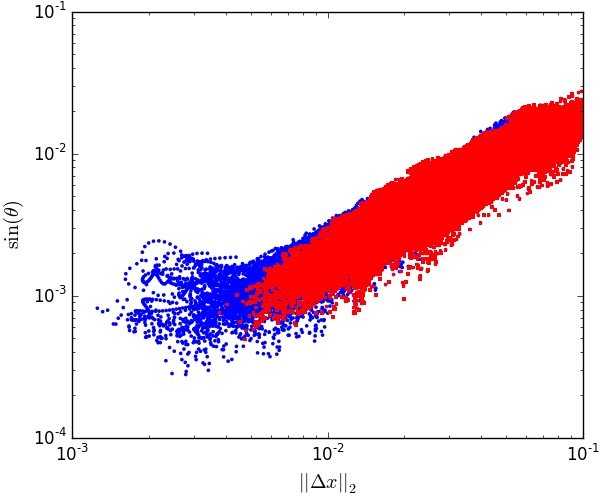
\includegraphics[width=0.45\textwidth]{disAngScatter_ppo3x10sT30}
    (d)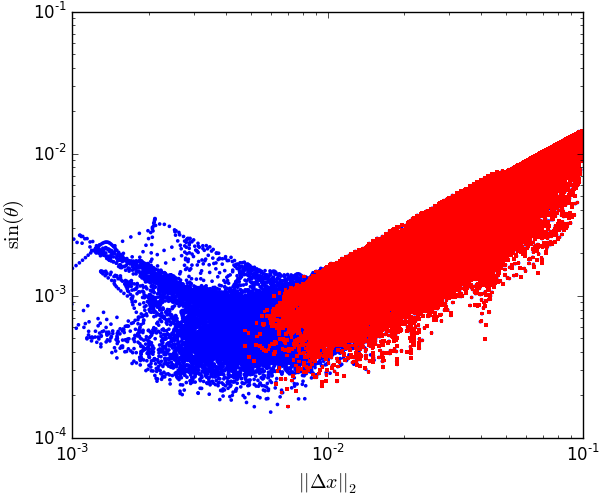
\includegraphics[width=0.45\textwidth]{disAngScatter_ppo4x10}
    (e)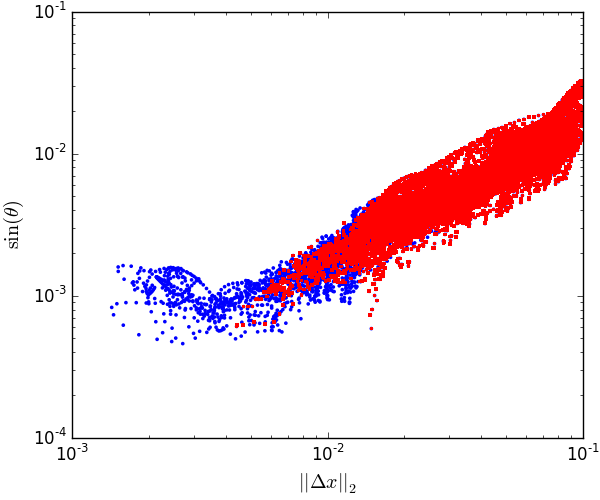
\includegraphics[width=0.45\textwidth]{disAngScatter_rpo1x10sT20}
    (f)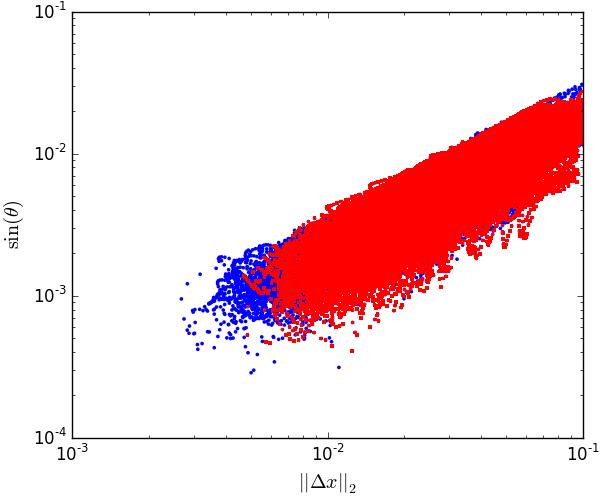
\includegraphics[width=0.45\textwidth]{disAngScatter_rpo3x10sT20}
    (g)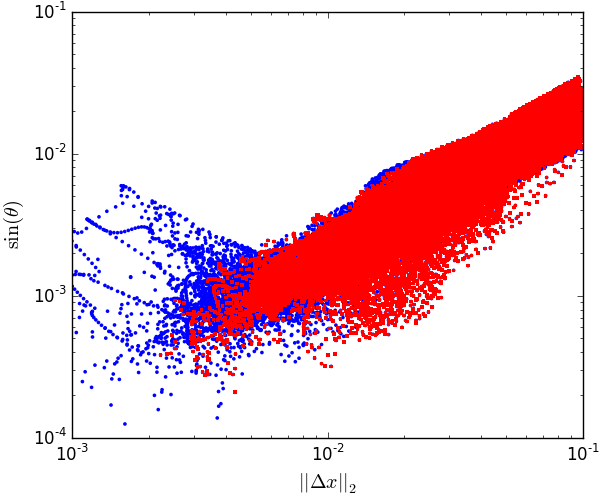
\includegraphics[width=0.45\textwidth]{disAngScatter_rpo4x10sT30}
    (h)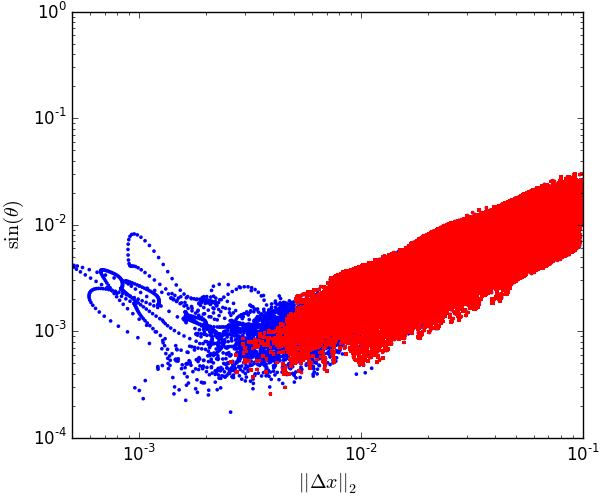
\includegraphics[width=0.45\textwidth]{disAngScatter_rpo6x10sT30}
    \caption{}
    \label{fig:disAngScatterN32_1}
  \end{figure}

 \begin{figure}[h]
   \centering
   (i)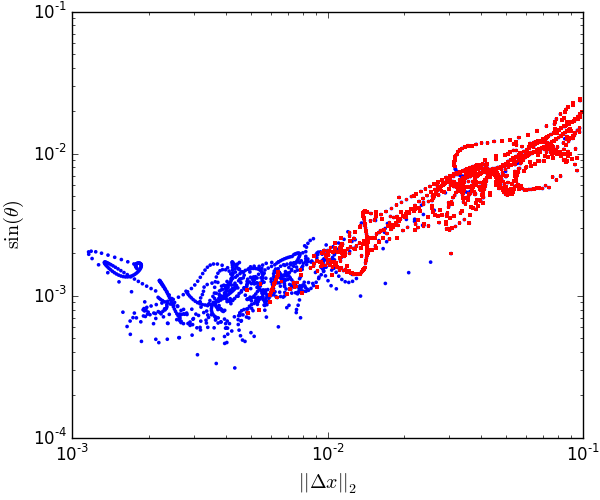
\includegraphics[width=0.45\textwidth]{disAngScatter_rpo8x10sT40}
   \caption{Combined with \reffig{fig:disAngScatterN32_1}.
     The blue dots are the raw data. The read dots are the shadowing
     points which satisfy relation :
     $||\Delta x_i||_2 > 4 \cdot S_i$. Where $S_i$ is the spacing between
     adjacent points in the PPO/RPO at location $i$.
     In the following,
     $T_p$ is the prime period of the orbit.
     $sT$ refers to the threshold shadowing time. $NI$ is the shadowing
     instances number. \\
     (a) \cycle{ppo1}, $T_p = 10.25$, $sT=20$, $NI=217$. \\
     (b) \cycle{ppo2}, $T_p = 14.33$, $sT=30$, $NI=1$.   \\
     (c) \cycle{ppo3}, $T_p = 32.36$, $sT=30$, $NI=198$. \\
     (d) \cycle{ppo4}, $T_p = 33.39$, $sT=30$, $NI=230$. \\
     (e) \cycle{rpo1}, $T_p = 16.31$, $sT=20$, $NI=66$.  \\
     (f) \cycle{rpo3}, $T_p = 33.50$, $sT=20$, $NI=560$. \\
     (g) \cycle{rpo4}, $T_p = 34.64$, $sT=30$, $NI=230$. \\
     (h) \cycle{rpo6}, $T_p = 36.22$, $sT=30$, $NI=751$. \\
     (i) \cycle{rpo8}, $T_p = 41.14$, $sT=40$, $NI=4$.   \\
   }
   \label{fig:disAngScatterN32_2}
  \end{figure}


\item[2015-2-27 Xiong Ding]
I updated figures  \reffig{fig:disAngScatterN32_1}
 \reffig{fig:disAngScatterN32_2}.
This time I add a constraint that the length of the difference vector
, which shadows point $x_i$ on the PPO/RPO, should be at least 4 times
larger than the spacing between adjacent points on the orbit at the
position $i$. Here, number 4 is chosen randomly.

I made this change because I think
the following scenario may be destructive
to the outcome: an ergodic trajectory is shadowing a part of PPO/RPO.
$x$ is a point in the ergodic trajectory and it is very close to
point $p_i$ on the PPO/RPO, but $p_i$ is far away from adjacent
points $p_{i+1}$ and $p_{i-1}$ on this
PPO/RPO, so actually, it is quite possible that $p_{i}$ is not the closest
point to $x$, but some other point between $p_i$ and $p_{i+1}$
(or $p_{i-1}$). Basically, it means that this PPO/RPO is not fine-grained.

The result shown in \reffig{fig:disAngScatterN32_1}
 \reffig{fig:disAngScatterN32_2} looks much better than the previous
ones. But this is just a crude filtering method, and it is prone to cut
away data at small distance. The next step, as suggested by Prof.
Predrag, is to use interpolation or local {\PoincSec} to rule out the
concern mentioned above.


\item[2015-2-28 Xiong]
  The spacing between adjacent points for \cycle{ppo4} and
  \cycle{rpo6} are shown in \reffig{fig:spacing_ppo4} and
  \reffig{fig:spacing_rpo6}. For both of them, the norm of the difference
  vector for two shadowing incidences
  are shown, and the oscillation parts are marked with letters.
  We retrieve the corresponding spacing along the RPO/PPO to see whether
  the oscillation is a consequence of large spacing in the orbit.
  The result basically confirms my assumption.

  For example, oscillation A in \reffig{fig:spacing_ppo4} corresponds
  to small spacing hill around index 4500-5000. And B, C and E
  correspond to the spike around 5900-6100.
  We also notice that if the ergodic trajectory is very close to
  the RPO/PPO, namely, $||\Delta x||_2$ is very small, slightly
  large spacing can result in oscillation; while when
  $||\Delta x||_2$ is relatively large, then only substantially large
  spacing, like the spikes in \reffig{fig:spacing_ppo4} and
  \reffig{fig:spacing_rpo6} is able to give birth to oscillation.

  \refFig{fig:spacing_ppo1rpo3} shows the spacing along two orbits,
  which have 'good' results in previous experiments. Panel (a) shows
  that the spacing is below $10^{-2}$, so that is why $\cycle{ppo1}$
  behaves well in the experiment. On the other hand, panel (b) shows
  that there is a large spike spacing along \cycle{rpo3}, so it
  should lead to bad experimental result. But \cycle{rpo3} behaves
  well from panel (f) of \reffig{fig:disAngScatterN32_1}. This
  confused me. I am not sure whether the reason is just luck.
  I check the percentage of shadowing points which satisfy
  relation $||\Delta x_i||_2 < 4 \cdot S_i$ and $||\Delta x_i||_2 < 5e-3$.
  \cycle{ppo4} has 3.85\%, while \cycle{rpo3} has less than 0.2\%.
  But certainly, there are ergodic trajectories which shadows \cycle{rpo3}
  for more than one period.

  \begin{figure}[h]
    \centering
    \includegraphics[width=\textwidth]{spacing_ppo4}
    \caption{
      spacing between adjacent points along orbit $\cycle{ppo4}$.
      It shows the spacing for $2T_p$ since we need to retrieve the part
      that is been shadowed by ergodic trajectories. (reflection symmetry
      is not reduced).
    }
    \label{fig:spacing_ppo4}
  \end{figure}

  \begin{figure}[h]
    \centering
    \begin{subfigure}[b]{0.48\linewidth}
      \centering
      \includegraphics[width=\textwidth]{oscillation_ppo4_1}
      \caption{}
      \label{fig:oscillation_ppo4_1}
    \end{subfigure}
    \hfill
    \begin{subfigure}[b]{0.48\linewidth}
      \centering
      \includegraphics[width=\textwidth]{oscillation_ppo4_2}
      \caption{}
      \label{fig:oscillation_ppo4_2}
    \end{subfigure}

    \caption{
      Two shadowing incidence for \cycle{ppo4} with
      shadowing time  $T\simeq 43$ and  $T\simeq 80$ respectively.
      Note, prime period is $T_p = 33.39$.
      Oscillation occurs at points $A$, $B$, $C$, $D$ and $E$, at
      which, the spacing in $\cycle{ppo4}$ approximately corresponds to
      index range 4575-4867, 5888-5998, 2570-2752, 4575-4848 and
      5888-6015 respectively in \reffig{fig:spacing_ppo4}.
    }
    \label{fig:oscillation_ppo4}
  \end{figure}

  \begin{figure}[h]
    \centering
    \includegraphics[width=\textwidth]{spacing_rpo6}
    \caption{
      spacing between adjacent points along orbit $\cycle{rpo6}$.
    }
    \label{fig:spacing_rpo6}
  \end{figure}

  \begin{figure}[h]
    \centering
    \begin{subfigure}[b]{0.48\linewidth}
      \centering
      \includegraphics[width=\textwidth]{oscillation_rpo6_1}
      \caption{}
      \label{fig:oscillation_rpo6_1}
    \end{subfigure}
    \hfill
    \begin{subfigure}[b]{0.48\linewidth}
      \centering
      \includegraphics[width=\textwidth]{oscillation_rpo6_2}
      \caption{}
      \label{fig:oscillation_rpo6_2}
    \end{subfigure}

    \caption{
      Two shadowing incidence for \cycle{rpo6} with
      shadowing time  $T\simeq 30$.
      Note, prime period is $T_p = 36.22$.
      Oscillation occurs at points $A$, $B$ and $C$, at
      which, the spacing in $\cycle{rpo6}$ approximately corresponds to
      index range 1280-1405, 416-520 and 1302-1395
      respectively in \reffig{fig:spacing_rpo6}.
    }
    \label{fig:oscillation_ppo4}
  \end{figure}

  \begin{figure}[h]
    \centering
    \begin{subfigure}[b]{0.48\linewidth}
      \centering
      \includegraphics[width=\textwidth]{spacing_ppo1}
      \caption{}
      \label{fig:spacing_ppo1}
    \end{subfigure}
    \hfill
    \begin{subfigure}[b]{0.48\linewidth}
      \centering
      \includegraphics[width=\textwidth]{spacing_rpo3}
      \caption{}
      \label{fig:spacing_rpo3}
    \end{subfigure}

    \caption{
      Spacing along \cycle{ppo1} and \cycle{rpo3}
    }
    \label{fig:spacing_ppo1rpo3}
  \end{figure}

\item[2015-2-28 Xiong] I just have a quick check of Prof. Predrag's
    suggestion that We need to integrate the ergodic trajectory to the
    {\PoincSec} determined by the velocity at points on PPO/RPO. This
    is reasonable, since {\PoincSec} determined by velocity is not
    enough to guarantee that the difference vector is fairly well
    extracted. You can easily formulate a curve to demonstrate my
    point. The problem is still the coarse-grained PPO/RPO itself. We
    still need to interpolate the orbit in order to eliminate large
    spacing along the orbit.


\begin{figure}[h]
  \centering
  \begin{subfigure}[b]{0.48\linewidth}
    \centering
    \includegraphics[width=\textwidth]{shadowing_ppo4_1}
    \caption{}
    \label{fig:shadowing_ppo4_1}
  \end{subfigure}
  \hfill
  \begin{subfigure}[b]{0.48\linewidth}
    \centering
    \includegraphics[width=\textwidth]{shadowing_ppo4_2}
    \caption{}
    \label{fig:shadowing_ppo4_1}
  \end{subfigure}

  \caption{
    Two segments of the same shadowing incidence for \cycle{ppo4}.
    (a) corresponds to the oscillating part A in \reffig{fig:oscillation_ppo4_1}.
    (b) corresponds to the immediate following part after A in \reffig{fig:oscillation_ppo4_1}.
    Blue dots belongs to ergodic trajectory. Dashed curve belongs to \cycle{ppo4}.
    Green dots are the corresponding shadowing points on \cycle{ppo4} by the blue dots.
    x, y axes are the real part of 1st and 2nd Fourier modes respectively.
    Be careful about the scale of x, y axis in order to determine the correct shadowing
    pair.
  }
  \label{fig:spacing_ppo1rpo3}
\end{figure}

\item[2015-3-17 Evangelos] As an alternative to interpolation you might want to try
the following: as soon as the distance falls bellow a prescribed threshold reduce time resolution for the integration
of the PPO/RPO to some small value integrating until the next point at the (coarser resolution) PPO/RPO.
Then take the next point on the (coarser resolution) PPO/RPO and integrate again with smaller stepsize etc.
I think that the error that you introduce this way will be very small for small segments of the orbit and this will allow you to
have a finelly resolved orbit in time for the relevant segments (without the need to refine the whole orbit). For the ergodic
trajectory do you already use some small time-step than you do for the RPO/PPO?

\item[2015-3-24 Xiong to Evangelos]
I am sorry I did not notice your reply. Your suggestion
is one way to resolve this problem, but I have not tried.
For the ergodic trajectory,
I use a large integration time step for efficiency. I think as long
as one orbit (periodic or ergodic) has small spacing, then
this problem will disappear.

Sorry to you guys that I did little on it for about one month.

\item[2015-5-3 Xiong]
Sorry for not working on this project for a long time. Today I tried
to use smaller integration time step to eliminate the blow-up
problem in our previous trial. The result is promising even though
I only tried one point on one shadowing incidence, but I will go
forward to apply it to our original data. The result is
in \href{matlab/angDist\_html/AngDist.html}{/lyapunov/matlab/angDist\_html/AngDist.html}.
(see the last figure)
\end{description}
